%%%%%%%%%%%%%%%%%%%%%%%%%%%%%%%%%%%%%%%%
% datoteka diploma-vzorec.tex
%
% vzorčna datoteka za pisanje diplomskega dela v formatu LaTeX
% na UL Fakulteti za računalništvo in informatiko
%
% vkup spravil Gašper Fijavž, december 2010
% 
%
%
% verzija 12. februar 2014 (besedilo teme, seznam kratic, popravki Gašper Fijavž)
% verzija 10. marec 2014 (redakcijski popravki Zoran Bosnić)
% verzija 11. marec 2014 (redakcijski popravki Gašper Fijavž)
% verzija 15. april 2014 (pdf/a 1b compliance, not really - just claiming, Damjan Cveta, Gašper Fijavž)

\documentclass[a4paper, 12pt]{book}

\usepackage[utf8x]{inputenc}   % omogoča uporabo slovenskih črk kodiranih v formatu UTF-8
\usepackage[slovene,english]{babel}    % naloži, med drugim, slovenske delilne vzorce
\usepackage[pdftex]{graphicx}  % omogoča vlaganje slik različnih formatov
\usepackage{fancyhdr}          % poskrbi, na primer, za glave strani
\usepackage{amssymb}           % dodatni simboli
\usepackage{amsmath}           % eqref, npr.
\usepackage{array}
%\usepackage{hyperxmp}
\usepackage[pdftex, colorlinks=true,
						citecolor=black, filecolor=black, 
						linkcolor=black, urlcolor=black,
						pagebackref=false, 
						pdfproducer={LaTeX}, pdfcreator={LaTeX}, hidelinks]{hyperref}



%%%%%%%%%%%%%%%%%%%%%%%%%%%%%%%%%%%%%%%%
%	DIPLOMA INFO
%%%%%%%%%%%%%%%%%%%%%%%%%%%%%%%%%%%%%%%%
\newcommand{\ttitle}{Implementacija metode asimetričnega srednjega drevesa za iskanje konsenza filogenetskih dreves}
\newcommand{\ttitleEn}{Diploma thesis sample}
\newcommand{\tsubject}{\ttitle}
\newcommand{\tsubjectEn}{\ttitleEn}
\newcommand{\tauthor}{Urban Soban}
\newcommand{\tkeywords}{konsenz, drevo, filogenetika}
\newcommand{\tkeywordsEn}{consensus, tree, phylogeny}



\usepackage{hyperref}
%%%%%%%%%%%%%%%%%%%%%%%%%%%%%%%%%%%%%%%%
%	HYPERREF SETUP
%%%%%%%%%%%%%%%%%%%%%%%%%%%%%%%%%%%%%%%%
\hypersetup{pdftitle={\ttitle}}
\hypersetup{pdfsubject=\ttitleEn}
\hypersetup{pdfauthor={\tauthor, u.soban@gmail.com}}
\hypersetup{pdfkeywords=\tkeywordsEn}


 


%%%%%%%%%%%%%%%%%%%%%%%%%%%%%%%%%%%%%%%%
% postavitev strani
%%%%%%%%%%%%%%%%%%%%%%%%%%%%%%%%%%%%%%%%  
\renewcommand{\baselinestretch}{1.3} % ustrezen razmik med vrsticami
\setlength{\headheight}{15pt}        % potreben prostor na vrhu
\renewcommand{\chaptermark}[1]%
{\markboth{\MakeUppercase{\thechapter.\ #1}}{}} \renewcommand{\sectionmark}[1]%
{\markright{\MakeUppercase{\thesection.\ #1}}} \renewcommand{\headrulewidth}{0.5pt} \renewcommand{\footrulewidth}{0pt}
\fancyhf{}
\fancyhead[LE,RO]{\sl \thepage} \fancyhead[LO]{\sl \rightmark} \fancyhead[RE]{\sl \leftmark}



\newcommand{\BibTeX}{{\sc Bib}\TeX}

%%%%%%%%%%%%%%%%%%%%%%%%%%%%%%%%%%%%%%%%
% naslovi
%%%%%%%%%%%%%%%%%%%%%%%%%%%%%%%%%%%%%%%%  


\newcommand{\autfont}{\Large}
\newcommand{\titfont}{\LARGE\bf}
\newcommand{\clearemptydoublepage}{\newpage{\pagestyle{empty}\cleardoublepage}}
\setcounter{tocdepth}{1}	      % globina kazala

%%%%%%%%%%%%%%%%%%%%%%%%%%%%%%%%%%%%%%%%
% konstrukti
%%%%%%%%%%%%%%%%%%%%%%%%%%%%%%%%%%%%%%%%  
\newtheorem{izrek}{Izrek}[chapter]
\newtheorem{trditev}{Trditev}[izrek]
\newenvironment{dokaz}{\emph{Dokaz.}\ }{\hspace{\fill}{$\Box$}}

%%%%%%%%%%%%%%%%%%%%%%%%%%%%%%%%%%%%%%%%%%%%%%%%%%%%%%%%%%%%%%%%%%%%%%%%%%%%%%%
%% PDF-A
%%%%%%%%%%%%%%%%%%%%%%%%%%%%%%%%%%%%%%%%%%%%%%%%%%%%%%%%%%%%%%%%%%%%%%%%%%%%%%%

%%%%%%%%%%%%%%%%%%%%%%%%%%%%%%%%%%%%%%%% 
% define medatata
%%%%%%%%%%%%%%%%%%%%%%%%%%%%%%%%%%%%%%%% 
\def\Title{\ttitle}
\def\Author{\tauthor, u.soban@gmail.com}
\def\Subject{\ttitleEn}
\def\Keywords{\tkeywordsEn}

%%%%%%%%%%%%%%%%%%%%%%%%%%%%%%%%%%%%%%%% 
% \convertDate converts D:20080419103507+02'00' to 2008-04-19T10:35:07+02:00
%%%%%%%%%%%%%%%%%%%%%%%%%%%%%%%%%%%%%%%% 
\def\convertDate{%
    \getYear
}

{\catcode`\D=12
 \gdef\getYear D:#1#2#3#4{\edef\xYear{#1#2#3#4}\getMonth}
}
\def\getMonth#1#2{\edef\xMonth{#1#2}\getDay}
\def\getDay#1#2{\edef\xDay{#1#2}\getHour}
\def\getHour#1#2{\edef\xHour{#1#2}\getMin}
\def\getMin#1#2{\edef\xMin{#1#2}\getSec}
\def\getSec#1#2{\edef\xSec{#1#2}\getTZh}
\def\getTZh +#1#2{\edef\xTZh{#1#2}\getTZm}
\def\getTZm '#1#2'{%
    \edef\xTZm{#1#2}%
    \edef\convDate{\xYear-\xMonth-\xDay T\xHour:\xMin:\xSec+\xTZh:\xTZm}%
}

\expandafter\convertDate\pdfcreationdate 

%%%%%%%%%%%%%%%%%%%%%%%%%%%%%%%%%%%%%%%%
% get pdftex version string
%%%%%%%%%%%%%%%%%%%%%%%%%%%%%%%%%%%%%%%% 
\newcount\countA
\countA=\pdftexversion
\advance \countA by -100
\def\pdftexVersionStr{pdfTeX-1.\the\countA.\pdftexrevision}


%%%%%%%%%%%%%%%%%%%%%%%%%%%%%%%%%%%%%%%%
% XMP data
%%%%%%%%%%%%%%%%%%%%%%%%%%%%%%%%%%%%%%%%  
\usepackage{xmpincl}
\includexmp{pdfa-1b}

%%%%%%%%%%%%%%%%%%%%%%%%%%%%%%%%%%%%%%%%
% code
%%%%%%%%%%%%%%%%%%%%%%%%%%%%%%%%%%%%%%%%  
\usepackage{color}
\usepackage{listings}

\definecolor{Code}{rgb}{0,0,0}
\definecolor{Decorators}{rgb}{0.5,0.5,0.5}
\definecolor{Numbers}{rgb}{0.5,0,0}
\definecolor{MatchingBrackets}{rgb}{0.25,0.5,0.5}
\definecolor{Keywords}{rgb}{0,0,1}
\definecolor{self}{rgb}{0,0,0}
\definecolor{Strings}{rgb}{0,0.63,0}
\definecolor{Comments}{rgb}{0,0.63,1}
\definecolor{Backquotes}{rgb}{0,0,0}
\definecolor{Classname}{rgb}{0,0,0}
\definecolor{FunctionName}{rgb}{0,0,0}
\definecolor{Operators}{rgb}{0,0,0}
\definecolor{Background}{rgb}{0.98,0.98,0.98}

\lstset{
	captionpos=b
}

\lstnewenvironment{python}[1][]{
\lstset{
	numbers=left,
	numberstyle=\footnotesize,
	numbersep=1em,
	xleftmargin=1em,
	framextopmargin=2em,
	framexbottommargin=2em,
	showspaces=false,
	showtabs=false,
	showstringspaces=false,
	frame=l,
	tabsize=4,
	% Basic
	basicstyle=\ttfamily\footnotesize,	
	%basicstyle=\ttfamily\footnotesize\setstretch{1},
	backgroundcolor=\color{Background},
	language=Python,
	% Comments
	commentstyle=\color{Comments}\slshape,
	% Strings
	stringstyle=\color{Strings},
	morecomment=[s][\color{Strings}]{"""}{"""},
	morecomment=[s][\color{Strings}]{'''}{'''},
	% keywords
morekeywords={import,from,class,def,for,while,if,is,in,elif,else,not,and,or,print,break,continue,return,True,False,None,access,as,,del,except,exec,finally,global,import,lambda,pass,print,raise,try,assert},
	keywordstyle={\color{Keywords}\bfseries},
	% additional keywords
	morekeywords={[2]@invariant},
	keywordstyle={[2]\color{Decorators}\slshape},
	emph={self},
	emphstyle={\color{self}\slshape},
	%
	captionpos=b,
	#1
}}{}
\renewcommand\lstlistingname{Koda}

%%%%%%%%%%%%%%%%%%%%%%%%%%%%%%%%%%%%%%%%
% pdfInfo
%%%%%%%%%%%%%%%%%%%%%%%%%%%%%%%%%%%%%%%%  
\pdfinfo{%
    /Title    (\ttitle)
    /Author   (\tauthor, u.soban@gmail.com)
    /Subject  (\ttitleEn)
    /Keywords (\tkeywordsEn)
    /ModDate  (\pdfcreationdate)
    /Trapped  /False
}


%%%%%%%%%%%%%%%%%%%%%%%%%%%%%%%%%%%%%%%%%%%%%%%%%%%%%%%%%%%%%%%%%%%%%%%%%%%%%%%
%%%%%%%%%%%%%%%%%%%%%%%%%%%%%%%%%%%%%%%%%%%%%%%%%%%%%%%%%%%%%%%%%%%%%%%%%%%%%%%

\begin{document}
\selectlanguage{slovene}
\frontmatter
\setcounter{page}{1} %
\renewcommand{\thepage}{}       % preprecimo težave s številkami strani v kazalu

%%%%%%%%%%%%%%%%%%%%%%%%%%%%%%%%%%%%%%%%
%naslovnica
 \thispagestyle{empty}%
   \begin{center}
    {\large\sc Univerza v Ljubljani\\%
      Fakulteta za računalništvo in informatiko}%
    \vskip 10em%
    {\autfont \tauthor\par}%
    {\titfont \ttitle \par}%
    {\vskip 2em \textsc{DIPLOMSKO DELO\\[2mm]
    UNIVERZITETNI ŠTUDIJSKI PROGRAM PRVE STOPNJE RAČUNALNIŠTVO IN INFORMATIKA}\par}%
    \vfill\null%
    {\large \textsc{Mentor}: doc.\ dr.  Tomaž Curk\par}%
    {\vskip 2em \large Ljubljana 2014 \par}%
\end{center}
% prazna stran
\clearemptydoublepage

%%%%%%%%%%%%%%%%%%%%%%%%%%%%%%%%%%%%%%%%
%copyright stran
\thispagestyle{empty}
\vspace*{8cm}
{\small \noindent
Rezultati diplomskega dela so intelektualna lastnina avtorja.
Za objavljanje ali izkoriščanje rezultatov di\-plom\-ske\-ga dela je potrebno pisno soglasje avtorja, Fakultete za ra\-ču\-nal\-niš\-tvo in
informatiko ter mentorja%
\footnote{V dogovorju z mentorjem lahko kandidat diplomsko delo s pripadajočo izvorno kodo izda tudi pod katero izmed alternativnih licenc, ki ponuja določen del pravic vsem: npr. Creative Commons, GNU GPL. V tem primeru na to mesto vstavite opis licence, na primer tekst~\cite{licence}.}.}


\begin{center}
\mbox{}\vfill
\emph{Besedilo je oblikovano z urejevalnikom besedil \LaTeX.}
\end{center}
% prazna stran
\clearemptydoublepage

%%%%%%%%%%%%%%%%%%%%%%%%%%%%%%%%%%%%%%%%
% stran 3 med uvodnimi listi
\thispagestyle{empty}
\vspace*{4cm}

\noindent
Fakulteta za računalništvo in informatiko izdaja naslednjo nalogo:
\medskip
\begin{tabbing}
\hspace{32mm}\= \hspace{6cm} \= \kill




Tematika naloge:
\end{tabbing}
Besedilo teme diplomskega dela študent prepiše iz študijskega informacijskega sistema, kamor ga je vnesel mentor. V nekaj stavkih bo opisal, kaj pričakuje od kandidatovega diplomskega dela. Kaj so cilji, kakšne metode uporabiti, morda bo zapisal tudi ključno literaturo.
\vspace{15mm}






\vspace{2cm}

% prazna stran
\clearemptydoublepage

%%%%%%%%%%%%%%%%%%%%%%%%%%%%%%%%%%%%%%%%
% izjava o avtorstvu
\vspace*{1cm}
\begin{center}
{\Large \textbf{\sc Izjava o avtorstvu diplomskega dela}}
\end{center}

\vspace{1cm}
\noindent Spodaj podpisani Urban Soban,
z vpisno številko \textbf{63100344}, sem avtor  diplomskega dela z naslovom:

\vspace{0.5cm}
\emph{Implementacija metode asimetričnega srednjega drevesa za iskanje konsenza filogenetskih dreves}

\vspace{1.5cm}
\noindent S svojim podpisom zagotavljam, da:
\begin{itemize}
	\item sem diplomsko delo izdelal samostojno pod mentorstvom
		doc.\ dr.\ Tomaža Curka

	\item	so elektronska oblika diplomskega dela, naslov (slov., angl.), povzetek (slov., angl.) ter ključne besede (slov., angl.) identični s tiskano obliko diplomskega dela,
	\item soglašam z javno objavo elektronske oblike diplomskega dela na svetovnem spletu preko univerzitetnega spletnega arhiva.	
\end{itemize}

\vspace{1cm}
\noindent V Ljubljani, dne 11. januarja 2011 \hfill Podpis avtorja:

% prazna stran
\clearemptydoublepage

%%%%%%%%%%%%%%%%%%%%%%%%%%%%%%%%%%%%%%%%
% zahvala
\thispagestyle{empty}\mbox{}\vfill\null\it%
Na tem mestu zapišite, komu se zahvaljujete za izdelavo diplomske naloge. Pazite, da ne boste koga pozabili. Utegnil vam bo zameriti. Temu se da izogniti tako, da pozabite na celo zahvalo.
\rm\normalfont

% prazna stran
\clearemptydoublepage

%%%%%%%%%%%%%%%%%%%%%%%%%%%%%%%%%%%%%%%%
% posvetilo
\thispagestyle{empty}\mbox{}{\vskip0.20\textheight}\mbox{}\hfill\begin{minipage}{0.55\textwidth}%
Družini.
\normalfont\end{minipage}

% prazna stran
\clearemptydoublepage

%%%%%%%%%%%%%%%%%%%%%%%%%%%%%%%%%%%%%%%%
% kazalo
\def\thepage{}% preprecimo tezave s stevilkami strani v kazalu
\tableofcontents{}


% prazna stran
\clearemptydoublepage

%%%%%%%%%%%%%%%%%%%%%%%%%%%%%%%%%%%%%%%%
% seznam kratic

\chapter*{Seznam uporabljenih kratic}

\begin{tabular}{l|p{6cm}|p{6cm}}
  {\bf kratica} & {\bf angleško} & {\bf slovensko} \\ \hline
  % after \\: \hline or \cline{col1-col2} \cline{col3-col4} ...
  {\bf AMT} & asymmetric median tree & asimetrično srednje drevo \\
  {\bf MIS} & maximum independent set & največja neodvisna množica \\
  {\bf UPGMA} & unweighted pair group method with arithmetic mean & neuteženo gručanje s pomočjo aritmetične sredine \\
  {\bf CDAO} & comparative data analysis ontology  & ontologija s primerjavo podatkov \\
\end{tabular}



% prazna stran
\clearemptydoublepage

%%%%%%%%%%%%%%%%%%%%%%%%%%%%%%%%%%%%%%%%
% povzetek
\addcontentsline{toc}{chapter}{Povzetek}
\chapter*{Povzetek}
V vzorcu je predstavljen postopek priprave diplomskega dela z uporabo okolja \LaTeX. Vaš povzetek mora sicer vsebovati približno 100 besed, ta tukaj je odločno prekratek.
\bigskip

\noindent\textbf{Ključne besede:} \tkeywords.
% prazna stran
\clearemptydoublepage

%%%%%%%%%%%%%%%%%%%%%%%%%%%%%%%%%%%%%%%%
% abstract
\selectlanguage{english}
\addcontentsline{toc}{chapter}{Abstract}
\chapter*{Abstract}
This sample document presents an approach to typesetting your BSc thesis using \LaTeX. A proper abstract should contain around 100 words which makes this one way too short.
\bigskip

\noindent\textbf{Keywords:} \tkeywordsEn.
\selectlanguage{slovene}
% prazna stran
\clearemptydoublepage

%%%%%%%%%%%%%%%%%%%%%%%%%%%%%%%%%%%%%%%%
\mainmatter
\setcounter{page}{1}
\pagestyle{fancy}

\chapter{Uvod}
O evolucijskih razmerjih med živimi ogranizmi se je prvi spraševal Charles Darwin, ko je narisal znamenito "drevo življenja", prikazano na sliki (\ref{img-darwin-tree}). Vendar je Darwin lahko organizme razvrščal le glede na njihove morfološke lastnosti. Nato je prišlo do odkritja DNA in izuma računalnika in porodila se je ideja o računski filogenetiki, eni izmed prvih področij bioinformatike, katere cilj je, predvsem iz sekvenc DNA in RNA, odkriti evolucijska razmerja med različnimi taksonomskimi enotami.  Mnoge računske filogenetske metode so bile razvite že v prejšnjem stoletju, vendar so nekatere v praktično uporabo prišle šele v zadnjem času zaradi eksponentnega povečanja računske moči. Ker različne metode ali pa celo ena sama metoda lahko proizvede več različnih filogenetskih dreves, mnogokrat želimo rezultate kombinirati v eno drevo in tako pridobiti eno teorijo o evolucijski zgodovini taksonomskih enot. 

Sem na pomoč priskočijo konsenzne metode, ki na podlagi različnih  kriterijev dele vhodnih dreves v končnem sestavljenem drevesu kombinirajo, ohranijo, ali zavržejo, s ciljem sestaviti drevo, katero kar se da dobro povzema informacije o evolucijski zgodovini, ki jih nosijo vhodna drevesa. Tekom konstrukcije konsenznega drevesa lahko metoda izračuna več različnih dreves, izbrano pa je tisto, ki uživa največjo podporo vhodnih dreves.

V prvem delu diplomske naloge se bomo na kratko seznanili z najbolj uporabljenimi metodami računanja filogenetskih dreves, katerih produkt je nato vhod v algoritem za izračun konsenza, in nato obravnavali nekatere priljubljene konsenzne metode, kot so striktni konsenz, večinski konsenz in srednji konsenz (konsenz mediane). V drugem delu naloge se bomo osredotočili na novejšo konsenzno metodo, algoritem asimetričnega srednjega drevesa. Spoznali bomo samo idejo algoritma in navedli njegove prednosti ter slabosti napram bolj uveljavljenim metodam. Sledilo bo teoretično ozadje konstrukcije asimetričnega srednjega drevesa, ki pa bo osvetljeno s strani praktične implementacije algoritma v programski paket Biopython. Za konec bomo teoretične prednosti in slabosti preizkusili eksperimentalno z uporabo dveh metrik za merjenje razrešenosti končnega filogenetskega drevesa.

\begin{figure}
	\begin{center}
		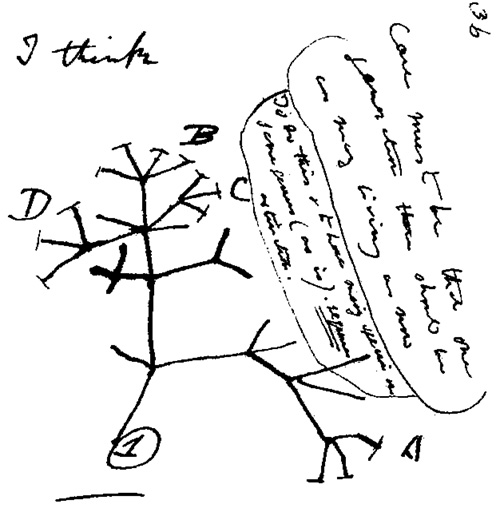
\includegraphics[scale=0.5]{gfx/darwin_tree.jpg}
	\end{center}
	\caption{"Drevo življenja", prva skica evolucijske zgodovine, narisana s strani Charlesa Darwina leta 1837\cite{cd}.}
	\label{img-darwin-tree}
\end{figure}


\chapter{Filogenetske in konsenzne metode}

V diplomski nalogi se povečamo konsenzni metodi asimetričnega srednjega drevesa. Da bi razumeli, zakaj so konsenzne metode v računski filogenetiki potrebne, bomo v tem razdelku zgolj na kratko predstavili, kako so filogenetska drevesa sploh zgrajena in kakšno vlogo pri tem igrajo konsenzne metode. 

\section{Filogenetske računske metode}

Filogenetske računske metode lahko razdelimo na dve večji skupini, distančne in statistične metode. Vse kot vhod prejmejo DNA ali RNA sekvence taksonomskih enot, katerih evolucijsko zgodovino želimo rekonstruirati, kot izhod pa vrnejo eno ali več filogenetskih dreves, ki imajo konice (liste) označene z imeni taksonomskih enot. Nekatere metode so zmožne oceniti tudi dolžino vej drevesa, pri čemer dolžina veje predstavlja čas, ki je bil potreben za divergenco dveh taksonomskih enot iz skupnega prednika. Izračun dolžin vej sicer ni odvisen zgolj od izbrane metode, temveč tudi od izbranega modela molekularne ure. Primere treh filogenetskih dreves za pet taksonomskih enot prikazuje slika \ref{img-input-trees}. Drevesa na sliki imajo dolžine vseh vej enake, med sabo pa se razlikujejo po topologiji.

\begin{figure}
	\begin{center}
		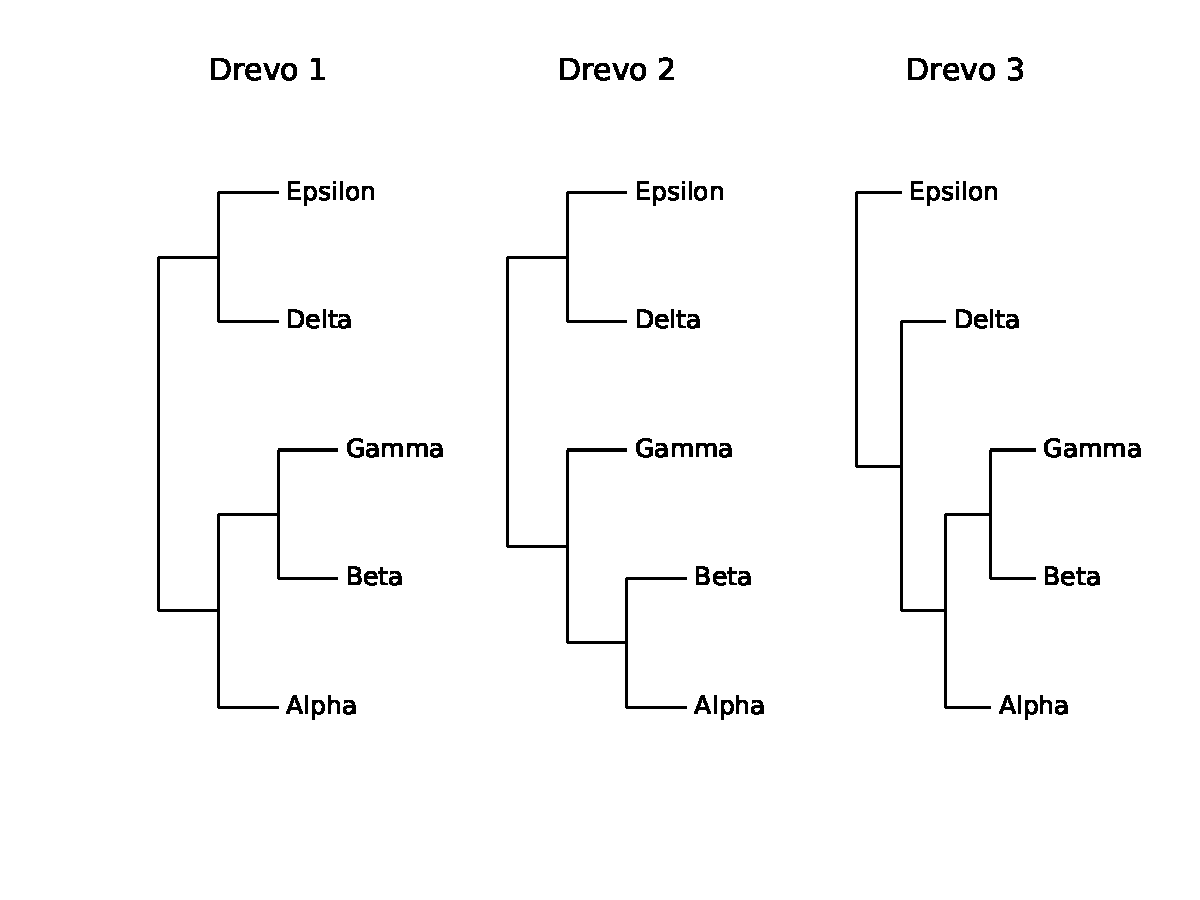
\includegraphics[scale=0.7, clip=true, trim=0 3cm 0 9mm]{gfx/input_trees_ex.pdf}
	\end{center}
	\caption{Primer treh filogenetskih dreves z različnimi topologijami.}
	\label{img-input-trees}
\end{figure}

\begin{itemize}
	\item distančne metode, katerim pripadata npr. UPGMA in algoritem najbližjih sosedov, za generiranje drevesa uporabljajo distančno matriko, ki je izračunana iz vhodnih sekvenc DNA ali RNA. V distančni matriki so zapisane razdalje med pari sekvenc in na njihovi podlagi algoritem v gruče uvršča po dve taksonomski enoti (oz. drugače povedano, dvema taksonomskima enotama določi skupnega prednika), dokler ni v gruče uvrstil vseh enot. Ko taksonomskih enot zmanjka, je drevo zgrajeno. Potrebno je omeniti, da te vrste metod delujejo deterministično in vrnejo le eno končno filogenetsko drevo.
	\item statistične metode, kot sta naprimer metodi maksimalnega verjetja in bayesova inferenca s pomočjo markovih verig, za razliko od distančnih metod uporabljajo statistične prijeme. Metoda maksimalnega verjetja išče drevo, pri katerem je verjetnost pojavitve podatkov (sekvenc) maksimalna, medtem ko bayesova metoda ocenjuje, koliko verjetni so dani podatki pri nekem drevesu. Te metode so bolj kompleksne in ponavadi dajajo boljše rezultate, vendar so se uveljavile šele v zadnjem času, saj so računsko precej bolj zahtevne.
\end{itemize}

Ker nobena izmed metod ne zagotavlja pravilno generirane evolucijske zgodovine oz. pravilnosti ne moremo preveriti (razen v primeru laboratorijskih organizmov, kjer je razmerje vnaprej znano)\cite{phy}, raziskovalci ponavadi najprej uporabijo eno izmed metod ponovnega vzorčenja, npr. jackknife ali bootstrap, s katero vzorčijo lokacije sekvenc in za vsak vzorec zgradijo svoje filogenetsko drevo. Vsako novo drevo se primerja s prvotno pridobljenim in oceni se delež bootstrapanih dreves, ki vsebujejo veje prvotnega drevesa. S pomočjo teh deležev lahko ocenimo, kolikšna je negotovost prvotno izračunane topologije filogenetskega drevesa\cite{fel}.   

Težava metod ponovnega vzorčenja je, da ocenjujejo zgolj negotovost v okviru ene metode. Raziskovalci lahko pridobijo več nasprotujočih si teorij o evolucijski zgodovini, naj si bo z uporabo različnih metod za računanje filogenetskega drevesa ali iz različnih virov podatkov. Ob tem se pojavi potreba po eni teoriji, ki bi kar se da dobro zajemala vse evolucijske dogodke, ki jih nosijo med sabo tekmujoče si teorije. To lahko dosežemo z uporabo konsenznih metod.

\section{Konsenzne metode}
Konsenzne metode nad filogenetskimi drevesi so uporabljene po vsakem filogenetskem algoritmu, ki kot izhod proizvede več filogenetskih dreves. Načeloma lahko delujejo nad katero koli množico dreves, v kateri imajo drevesa enake množice oznak listov. V tem se bistveno razlikujejo od metod super-dreves, katere so sposobne kombinirati tudi drevesa, katerih množice oznak listov niso enake\cite{bw}. Poleg metode asimetričnega srednjega drevesa, ki jo obravnavamo v nadaljevanju tega dela, naštejmo nekatere najbolj pogoste konsenzne metode:

\begin{itemize}
	\item kompatibilno drevo je sestavljeno iz delov vseh vhodnih dreves; ni nujno, da za vhodno množico dreves kompatibilno drevo dejansko tudi obstaja\cite{pw},
	\item striktni konsenz je najbolj konzervativna metoda, saj v končnem drevesu ohrani le tiste dele dreves, ki so prisotni v vseh drevesih vhodne množice\cite{bw}. Primer striktnega konsenznega drevesa za vhodna drevesa iz slike \ref{img-input-trees} je prikazan na sliki \ref{img-strict-majority-amt-example},
	\item večinski konsenz vsebuje le tiste dele drevesa, ki so prisotni v več kot polovici dreves vhodne množice\cite{bw}. Primer večinskega konsenznega drevesa za vhodna drevesa iz slike \ref{img-input-trees} je prikazan na sliki \ref{img-strict-majority-amt-example},
	\item srednji konsenz oz. mediana je drevo, ki minimizira vsoto simetričnih razlik glede na drevesa v vhodni množici. Večinsko drevo je prav tako srednje drevo, kar pomeni, da vedno obstaja vsaj eno srednje drevo\cite{pw}.
\end{itemize}

\begin{figure}[h!]
	\begin{center}
		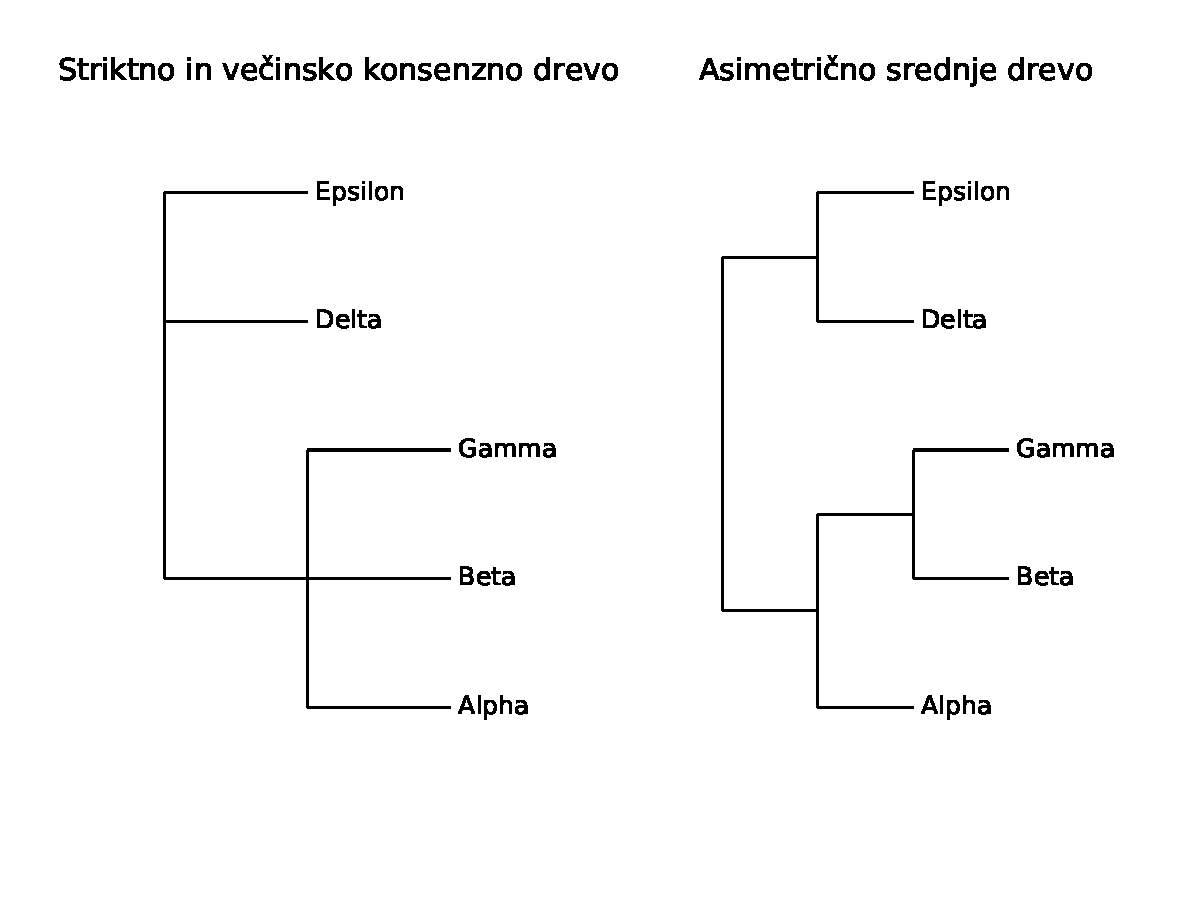
\includegraphics[scale=0.65, clip=true, trim=0 3cm 0 9mm]{gfx/strict_majority_amt_ex.pdf}
	\end{center}
	\caption{Na levi strani je prikazano striktno in večinsko konsenzno drevo za vhodna drevesa iz slike \ref{img-input-trees}. Drevesi sta v tem primeru enaki. Na desni je za isto vhodno množico prikazano asimetrično srednje drevo.}
	\label{img-strict-majority-amt-example}
\end{figure}

Večina konsenznih metod ignorira dolžine vej v vhodnih drevesih, tudi če so te navedene. Namen konsenznih metod je torej pridobiti topologijo drevesa, s katero se čim bolj strinjajo vhodna drevesa, ne pa tudi usklajevanje divergentnih časov taksonomskih enot in njihovih skupnih prednikov.  

\chapter{Asimetrično srednje drevo}
Metoda asimetričnega srednjega drevesa je nastala ob opažanju, da navadno srednje drevo kaznuje tiste dele dreves, ki ne nastopajo vsaj v polovici dreves vhodne množice, čeprav bi bilo smotrno, da se uporabi kar se da veliko informacije iz vseh vhodnih dreves\cite{pw}.

Metoda kot vhod prejme množico $k$ filogenetskih dreves $T = \left\{ {T_1, T_2, ..., T_k} \right\}$, katera imajo liste označene z $n$ taksonomskimi enotami iz množice $S = \left\{ {s_1, s_2, ..., s_n} \right\}$. Sledijo naslednji koraki algoritma, katerega dele bomo podrobneje obravnavali v naslednjih poglavjih:
\begin{itemize}
	\item drevesa pretvorimo v primerno reprezentacijo
	\item poiščemo nekompatibilne pare poddreves in konstruiramo graf nekompatibilnosti
	\item v grafu nekompatibilnosti poiščemo največjo neodvisno množico vozlišč
	\item rekonstruiramo drevo iz vozlišč največje neodvisne množice
\end{itemize}

\section{Kodiranje dreves}
Izbira predstavitve drevesa je pomembna za njihovo nadaljno manipulacijo. Izhajamo iz opažanja, da vsak rob drevesa, $e \in E(T_i)$, drevo razdeli na dva dela oz. particiji. Do vsakega lista (taksonomske enote $s$) vodi enolična pot, predstavljena z množico robov, ki na tej poti nastopajo. Označimo jo s $\pi(s)$. Nato definiramo preslikavo dveh argumentov (\ref{eq:1}), ki zavzame vrednost 1 v kolikor pot do podanega lista poteka preko podanega roba, sicer pa 0. $c(e, s)$ za vsak rob $e \in E(T_i)$ torej definira biparticijo drevesa $T_i$ \cite{pw}. V prvi množici so listi, do katerih lahko pridemo, če pot vodi preko roba $e$, v drugi pa tisti, do katerih v tem primeru ne moremo.

\begin{align}
	c(e, s) = 
	\left\{
		\begin{array}{ll}
			1 & e \in \pi(s) \\
			0 & e \notin \pi(s)
		\end{array}
	\right.
	\label{eq:1}
\end{align}

Vsak rob drevesa določa poddrevo, vendar nas ne bo zanimala celotna struktura poddreves, temveč zgolj njihovi listi. Liste poddrevesa z drugo besedo imenujemo klada (angl. clade). Vsako klado drevesa lahko predstavimo z binarnim nizom, ki ga dobimo z uporabo preslikave \ref{eq:2}, pri čemer je potrebno povdariti, da je vrstni red posameznih znakov v binarnem nizu pomemben, saj je na vsak znak vezan pomen; vsako posamezno mesto v nizu pripada enemu izmed listov drevesa, znak na tem mestu pa zgolj indicira prisotnost ali neprisotnost lista oz. taksonomske enote v kladi, kodirani z binarnim nizom.


\begin{align}
	c_e = \left\{ c(e, s): s \in S \right\} \label{eq:2}
\end{align}

V kolikor binarne nize vseh klad drevesa zberemo v množico (\ref{eq:3}), nam $C(T_i)$ določa kodiranje celotnega drevesa $T_i$. Primer dveh takih množic je prikazan na sliki \ref{img-bistring-trees-example}, kjer so binarni nizi prikazani na vejah, ki vodijo do korenov klad.

\begin{align}
	C(T_i) = \left\{ c_e : e \in E(T_i) \right\} \label{eq:3}
\end{align}

Kodiranje sedaj lahko izvedemo nad vsemi drevesi vhodne množice $T$, pri čemer je ponovno potrebno povdariti, da se pomen posameznih mest v binarnih nizih med različnimi drevesi ne sme spreminjati, saj sicer klad iz različnih dreves ne bi mogli medsebojno primerjati. 

\begin{figure}
	\begin{center}
		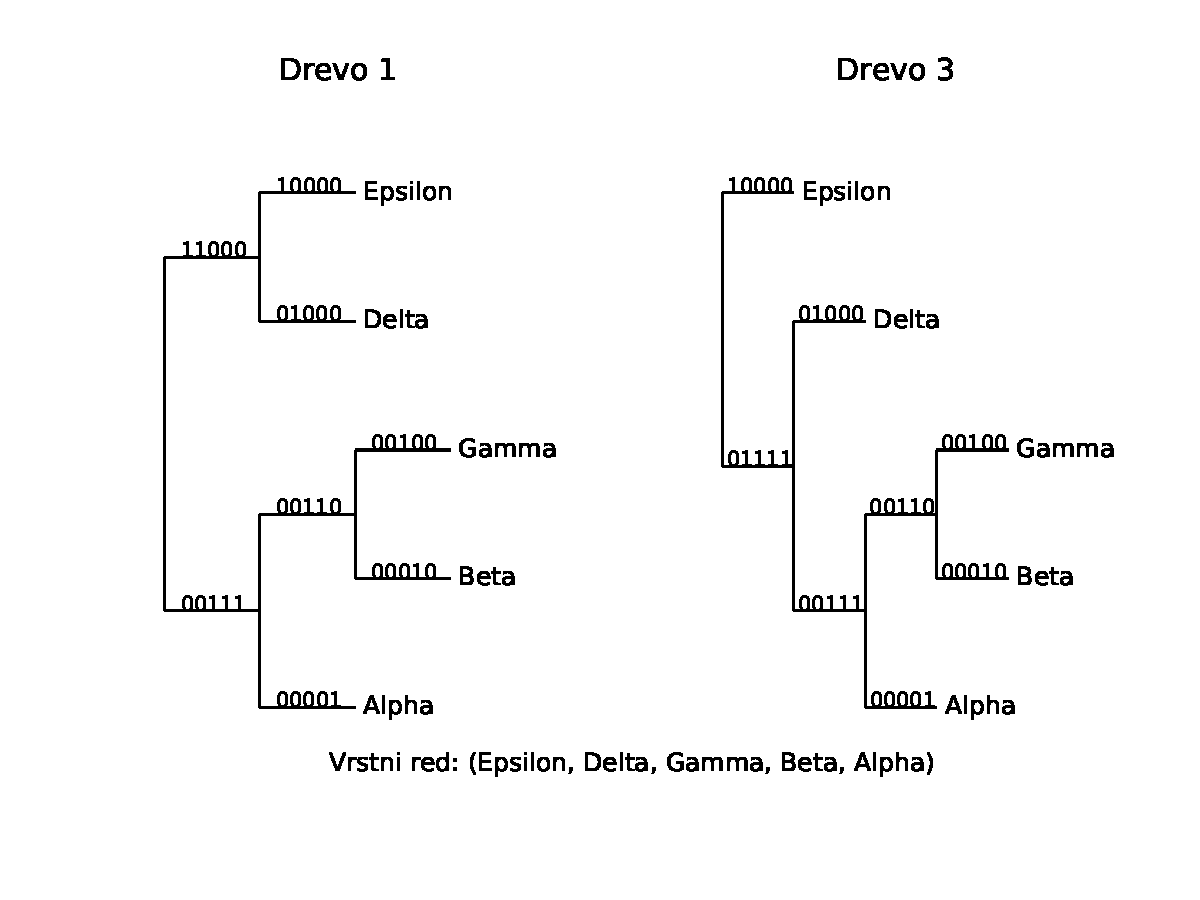
\includegraphics[scale=0.7, clip=true, trim=0 2cm 0 9mm]{gfx/bitstring_trees.pdf}
	\end{center}
	\caption{Vsi binarni nizi za prvo in tretje drevo iz slike \ref{img-input-trees}.}
	\label{img-bistring-trees-example}
\end{figure}

\section{Kompatibilnost binarnih nizov} 
Za konstrukcijo grafa nekompatibilnosti najprej potrebujemo kriterij kompatibilnosti klad oz. binarnih nizov, ki jih kodirajo. Za potrebe lažje predstavitve kompatibilnosti za vsak binarni niz $c_e$ definiramo množico $\phi(c_e)$ (\ref{eq:4}), ki vsebuje oznake taksonomskih enot, prisotnih v kladi oz. njenem pripadajočem binarnem nizu $c_e$. 

\begin{align}
	\phi(c_e) = c_e^{-1}(1) = \left\{ s \in S: c(e, s) = 1 \right\} \label{eq:4} \\
	\phi(j) \cap \phi(k) = \emptyset \lor \phi(j) \subseteq \phi(k) \lor \phi(k) \subseteq \phi(j) \label{eq:5}
\end{align} 

Če za binarna niza $j$ in $k$ iz poljubnih dveh dreves vhodne množice $T$ velja pogoj \ref{eq:5}, potem sta binarna niza kompatibilna. Vennov diagram pripadajočih množic $\phi(j)$ in $\phi(k)$ prikazuje slika \ref{img-venn-compatibility}. V kolikor velja $\left|\phi(j)\right| = 1$ ali $\left|\phi(k)\right| = 1$, potem sta binarna niza $j$ in $k$ vedno kompatibilna.   

\begin{figure}
	\begin{center}
		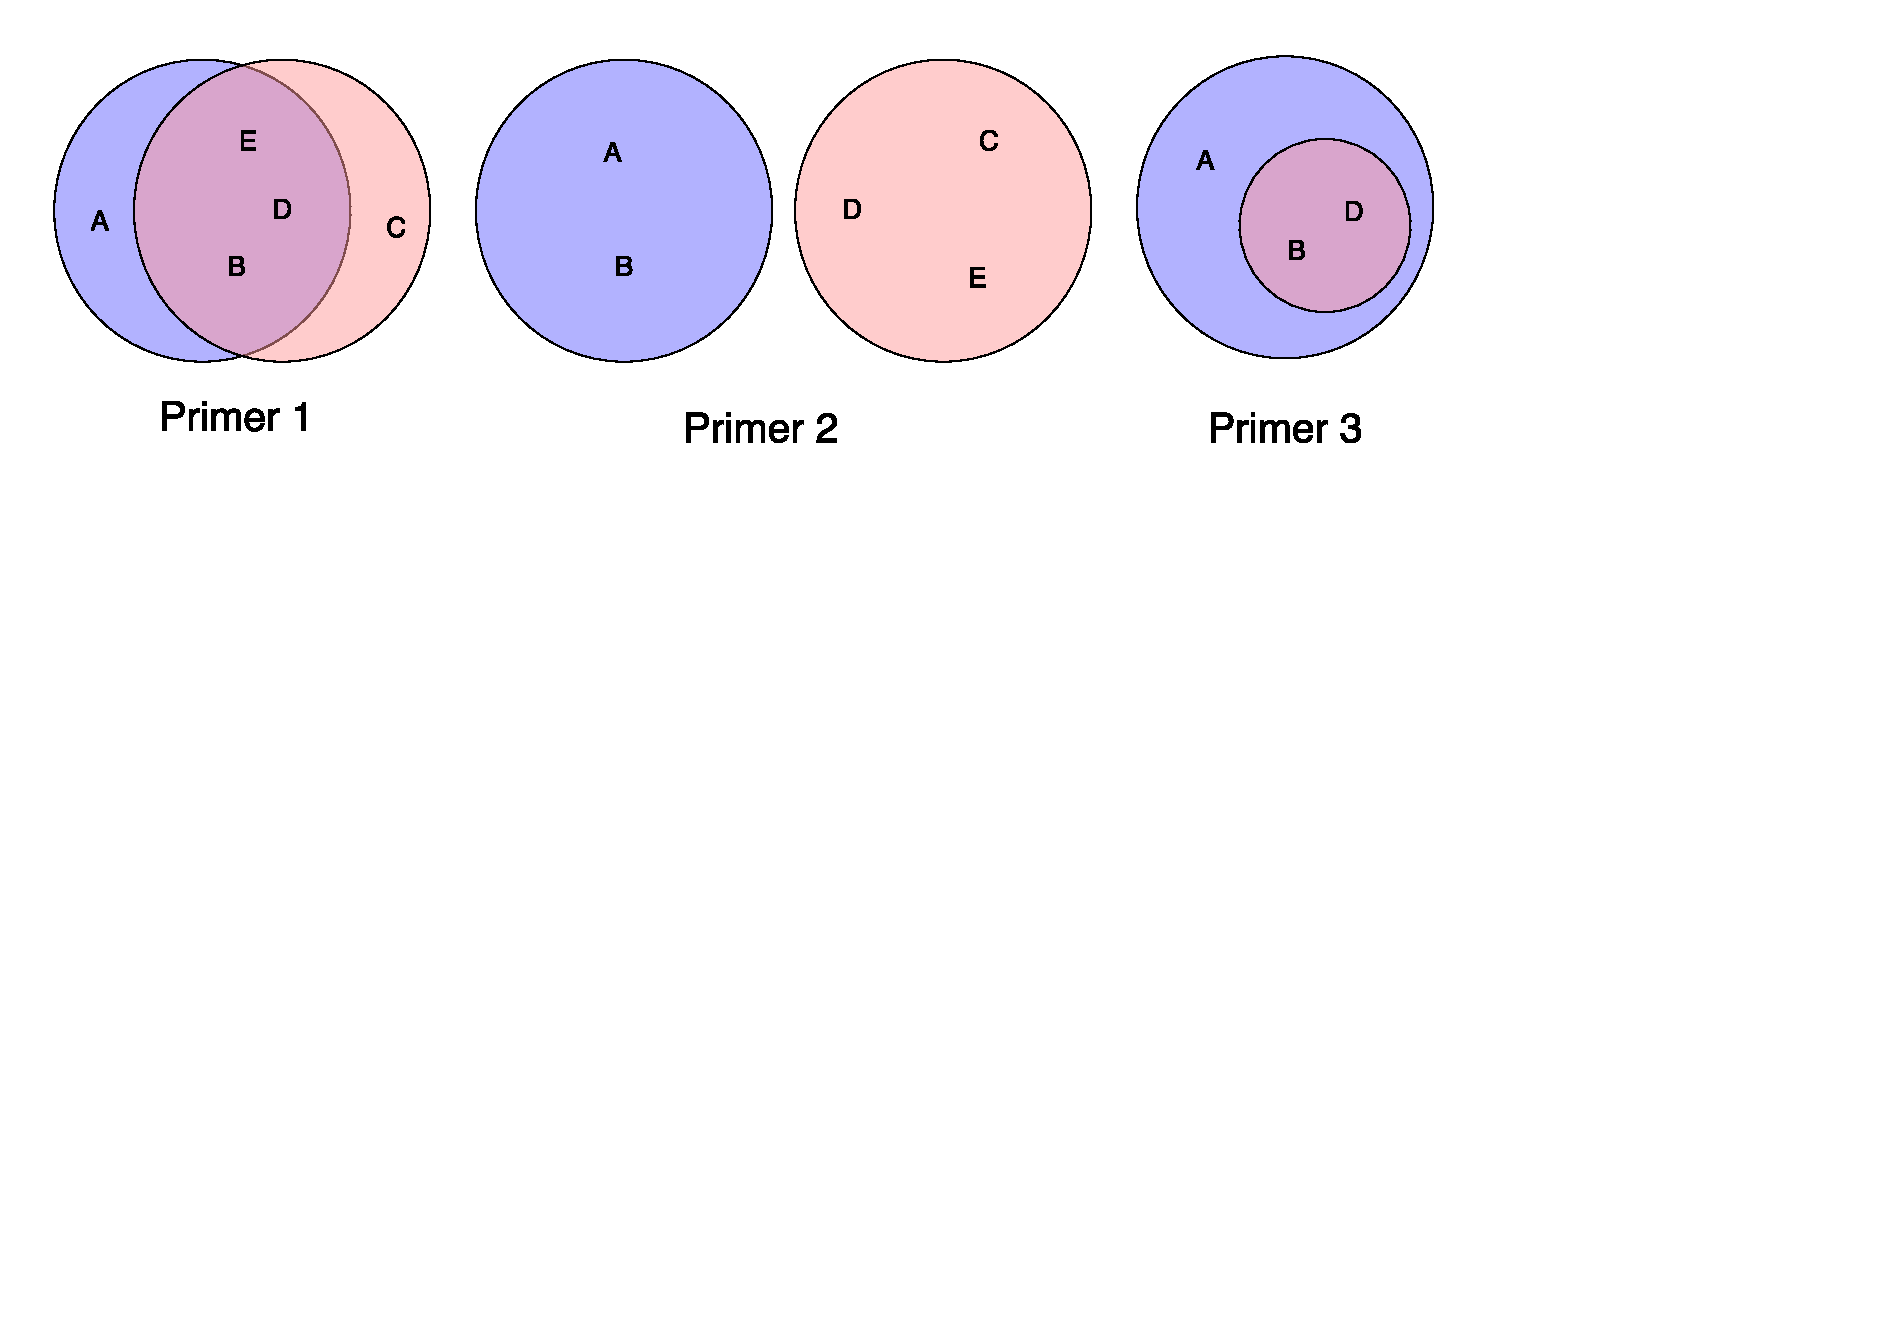
\includegraphics[scale=0.54, clip=true, trim=0 15cm 0 0]{gfx/venn-amt-compatibility.pdf}
	\end{center}
	\caption{Primera 2 in 3 prikazujeta kompatibilni množici $\phi$, v primeru 1 pa sta množici nekompatibilni.}
	\label{img-venn-compatibility}
\end{figure}

V kolikor kompatibilnost klad interpretiramo v smislu filogenetskega drevesa, potem posamezna klada predstavlja poddrevo s korenom, ki je notranje vozlišče drevesa $T_i$. Notranje vozlišče filogenetskega drevesa predstavlja skupnega prednika vsem vozliščem v poddrevesu pod njim. Nekompatibilni sta tisti poddrevesi, ki trdita, da se je iz obeh skupnih prednikov razvilo nekaj skupnih taksonomskih enot, a je hkrati v vsaj enem poddrevesu prisotna taksonomska enota, ki je v drugem poddrevesu ni. V tem primeru poddrevesi torej ponujata nasprotujoči si informaciji o evolucijski zgodovini. 

\section{Graf nekompatibilnosti}
Z uporabo kriterija nekompatibilnosti binarnih nizov lahko zgradimo graf nekompatibilnosti $I(V_1, V_2, ..., V_k, E) = I(V, E)$. Vsaka množica vozlišč $V_i$ predstavlja binarne nize $C(T_i)$, povezave v grafu pa vzpostavimo med tistimi vozlišči, katerih pripadajoči binarni nizi so med sabo nekompatibilni\cite{pw}. S povezovanjem vozlišč označimo binarne nize, ki v končnem drevesu skupaj ne morejo biti prisotni, sicer bi filogenetsko drevo podajalo dvoumne informacije o evolucijski zgodovini. 

Graf nekompatibilnosti vseh treh vhodnih dreves iz slike \ref{img-input-trees} je prikazan na sliki \ref{img-incompat-graph-example}. V prvem in drugem drevesu sta medsebojno nekompatibilni kladi $(Gamma, Alpha)$ in $(Gamma, Beta)$. Drevesi ponujata nasprotujoči si informaciji - prvo za najbolj sorodno taksonomski enoti $Gamma$ ponuja taksonomsko enoto $Alpha$, drugo pa taksonomsko enoto $Beta$. Prvo in drugo drevo imata medsebojno kompatibilni kladi $(Epsilon, Delta)$, ki pa sta nekompatibilni s klado $(Delta, Gamma, Beta, Alpha)$ iz tretjega vhodnega drevesa. Medtem ko prvo in drugo drevo trdita, da imata taksonomski enoti $Epsilon$ in $Delta$ neposrednega skupnega prednika, tretje drevo temu nasprotuje.

\begin{figure}
	\begin{center}
		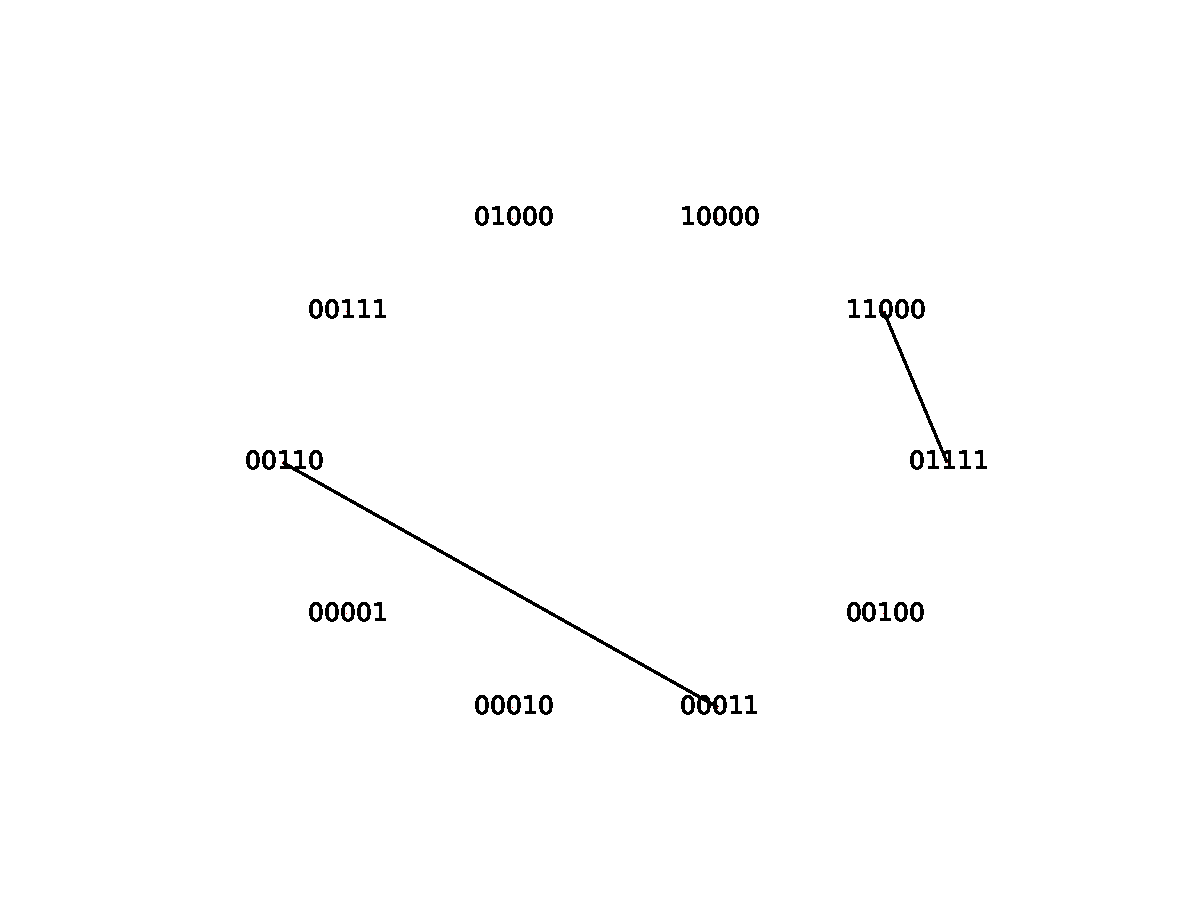
\includegraphics[scale=0.7, clip=true, trim=2cm 2cm 2cm 2cm]{gfx/incompat_graph.pdf}
	\end{center}
	\caption{Graf nekompatibilnosti biznih nizov za vhodna drevesa iz slike \ref{img-input-trees}. Vozlišča predstavljajo unikatne binarne nize iz vseh dreves vhodne množice $T$, povezave pa so vzpostavljene med pari vozlišč, katerih binarni nizi medsebojno niso kompatibilni.}
	\label{img-incompat-graph-example}
\end{figure}

\section{Največja neodvisna množica}
Graf nekompatibilnosti vsebuje vse informacije, ki jih potrebujemo za izbiro binarnih nizov, ki bodo prisotni v končnem filogenetskem drevesu. Vanj želimo vključiti kar se da veliko informacij, prisotnih v drevesih vhodne množice $T$. Najprej je potrebno zagotoviti, da vključimo binarne nize, ki so skupni vsem vhodnim drevesom $T_i$ (drevo, ki bi vsebovalo le te binarne nize, bi bilo striktno konsenzno drevo). Obenem želimo vključiti čimveč preostalih binarnih nizov, vendar ne takih, da bi bil katerikoli par nekompatibilen. 

Matematično orodje, ki nam iz grafa $I(V, E)$ omogoča izbiro vozlišč, ki paroma ne bodo kršile pogoja nekompatibilnosti, se imenuje neodvisna množica (angl. independent set). Neodvisna množica grafa je katerakoli množica vozlišč $V_{Indep} \subseteq V$, med katerimi ni medsebojnih povezav. Največja neodvisna množica grafa (angl. maximum independent set - MIS) je tista neodvisna množica $V_{MIS} \subseteq V$, ki vsebuje največ vozlišč. Potrebno je povdariti, da za nek graf $I(V, E)$ lahko obstaja več različnih $V_{MIS}$. Ker vozlišča $V_{MIS}$ predstavljajo binarne nize oz. klade končnega drevesa, to pomeni, da za en graf $I(V, E)$ lahko obstaja več asimetričnih srednjih dreves.

\begin{figure}
	\begin{center}
		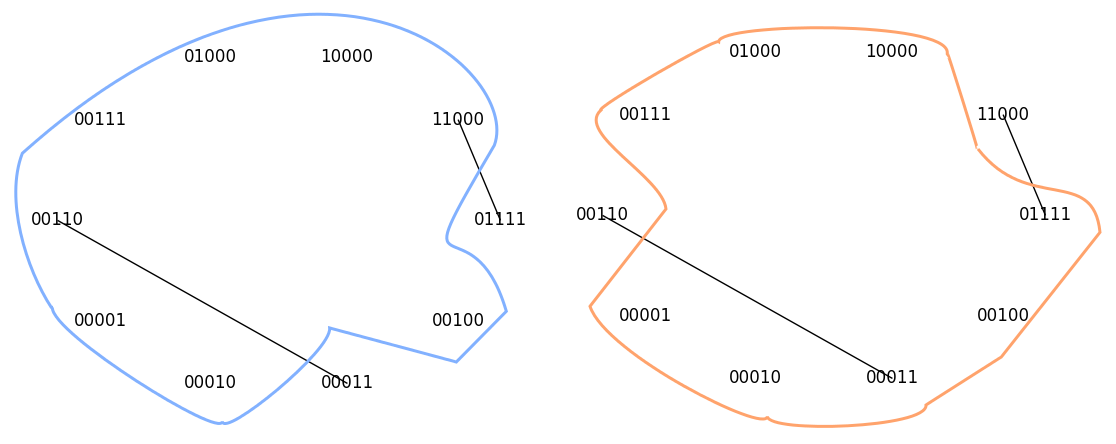
\includegraphics[scale=0.46]{gfx/incompat_graphs_pair.png}
	\end{center}
	\caption{Dve različni največji neodvisni množici za graf nekompatibilnosti iz slike \ref{img-incompat-graph-example}. Na danem grafu sicer obstajajo štiri največje neodvisne množice.}
	\label{img-mis-examples}
\end{figure}

Vozlišča grafa $I(V, E)$, katerega sestavimo iz $k$ dreves vhodne množice $T$, sestavljajo neodvisne množice $V_1, V_2, ..., V_k$. Vozlišča znotraj ene množice nikoli niso medsebojno povezana, saj njihovi pripadajoči binarni nizi pripadajo istemu drevesu. Vozlišči iz različnih množic pa lahko tvorita povezavo, v kolikor sta nekompatibilni. Tak graf imenujemo tudi k-partitni graf. Za bipartitne grafe obstaja trivialen polinomski algoritem s časovno zahtevnostjo $O(n^2)$, v splošnem pa problem največje neodvisne množice za k-partitne grafe sodi v razred NP-težkih algoritmov\cite{pw}. 

\section{Rekonstrukcija drevesa}
S tem, ko smo določili največjo neodvisno množico $V_{MIS}$ grafa $I(V, E)$, smo določili klade končnega drevesa, katerega strukturo pa je potrebno še rekonstruirati iz izbranih binarnih nizov. Problem rekonstrukcije evolucijske zgodovine $n$ taksonomskih enot iz njihovih binarnih nizov je dobro znan in se imenuje problem filogenije. Zanj obstaja algoritem s časovno kompleksnostjo $O(nm)$, pri čemer je $n$ število taksonomskih enot, $m$ pa število binarnih nizov v največji neodvisni množici\cite{gd}.

Najprej kreiramo matriko M dimenzij $n×m$. Binarne nize, ki pripadajo vozliščem množice $V_{MIS}$ kot stolpce zložimo v matriko $M$. Nato stolpce interpretiramo kot števila v binarnem zapisu, jih pretvorimo v desetiško obliko in sortiramo. Odstranimo stolpce s podvojeno vrednostjo, tako da ostanejo le stolpci z unikatnimi števili. S tem pridobimo matriko $M'$.

\begin{figure}
	\begin{center}
		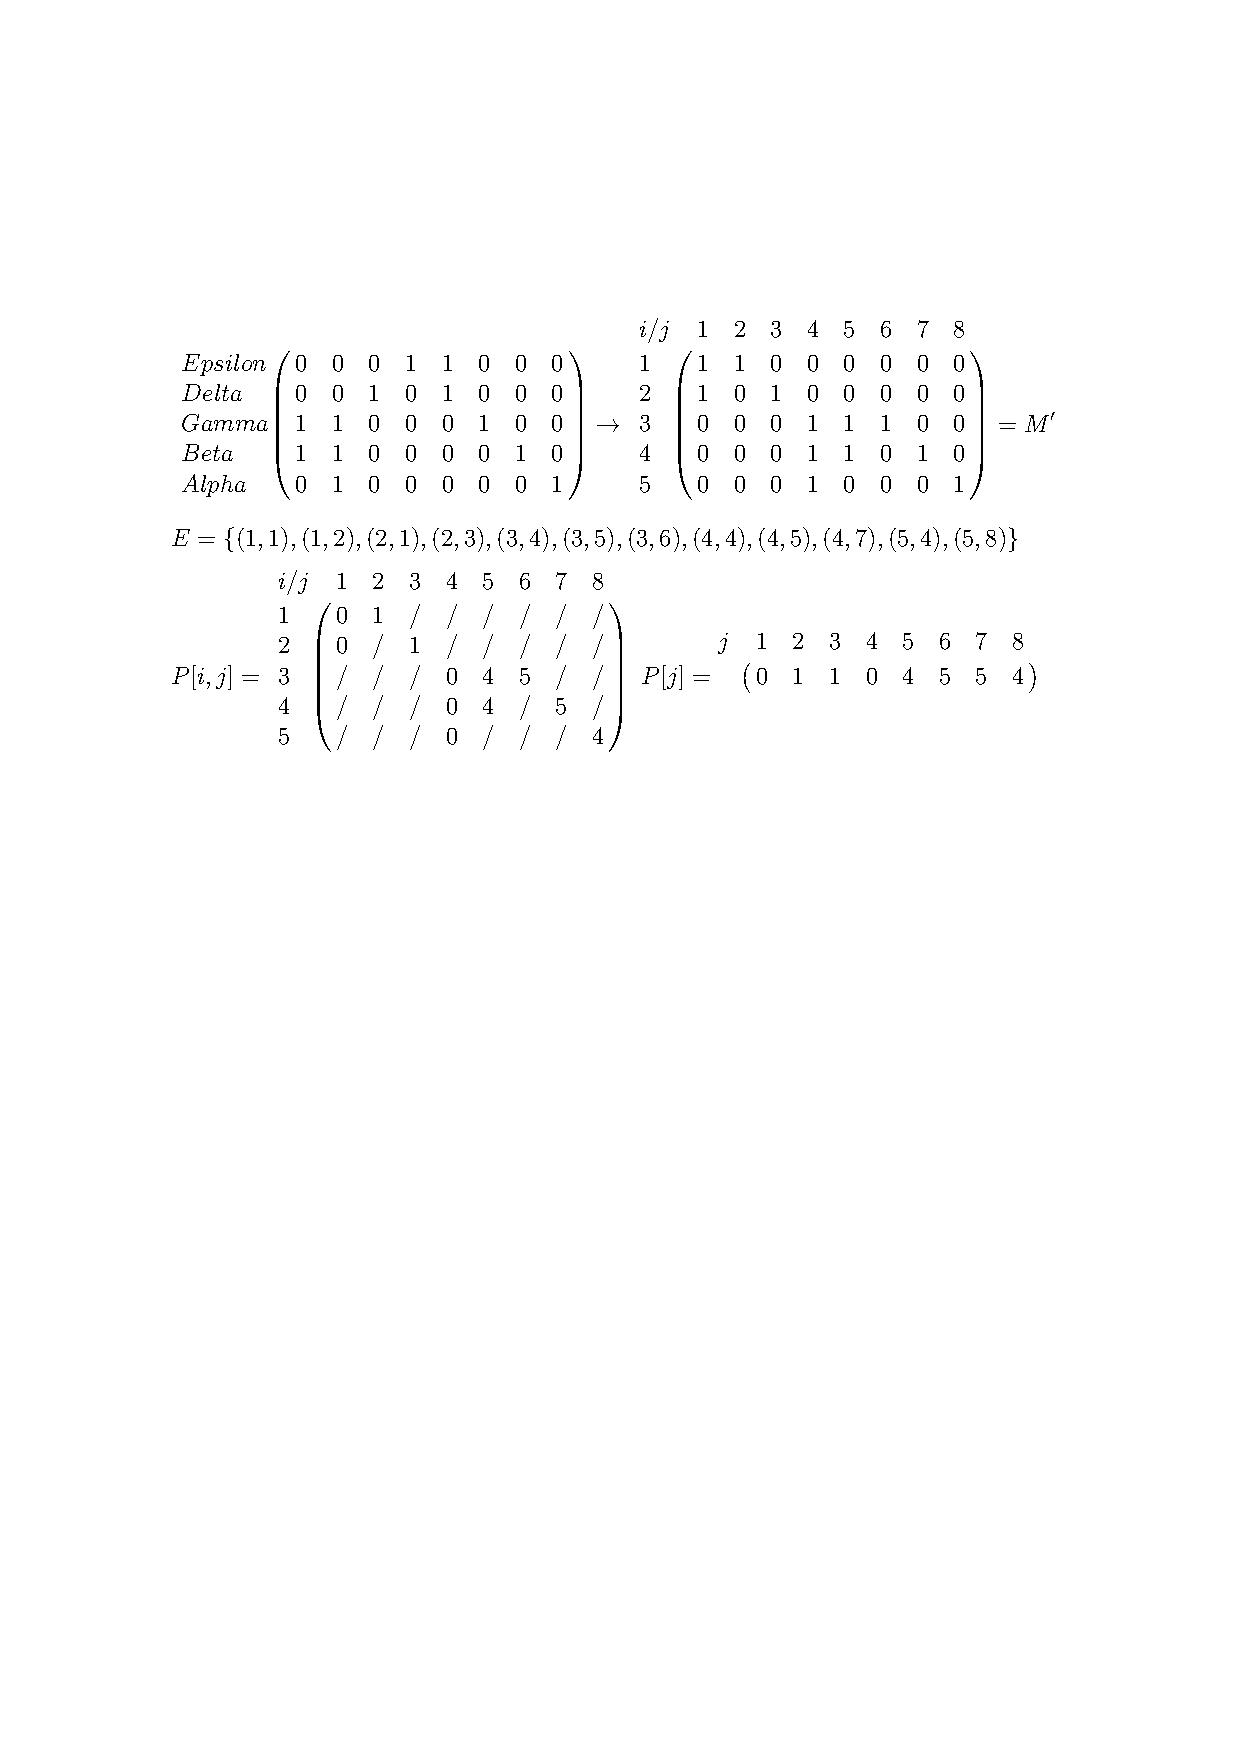
\includegraphics[scale=0.8, clip=true, trim=2.9cm 17cm 3cm 5cm]{gfx/tree_reconstruction_m.pdf}
	\end{center}
	\caption{Primer izračuna matrike $M'$, množice parov indeksov $E$ in vseh vrednosti $P(i, j)$ ter $P(j)$ za prvo največjo neodvisno množico iz slike \ref{img-mis-examples}. Ker enačba \ref{eq:9} v tem primeru velja, iz matrike $M'$ lahko zgradimo filogenetsko drevo.}
	\label{img-reconstruct-m}
\end{figure}

Naj bo $I_i$ množica indeksov vrstic, $I_j$ pa množica indeksov stolpcev matrike $M'$. Množica $E$ (\ref{eq:6}) predstavlja vse pare indeksov $(i, j) \in I_i \times I_j$ matrike $M'$, katerih vrednost je enaka ena.

\begin{align}
	E = \left\{ {(i, j): i \in I_i, j \in I_j, M'(i, j) = 1} \right\} \label{eq:6} \\
	P(i, j) = 
		\left\{
		\begin{array}{ll}
			\max(\left\{k: (i, k) \in E, k < j\right\}) \\
			0 $      "ce tak $k$ ne obstaja$
		\end{array}
		\right.
	\label{eq:7}
\end{align}

Vsak par $(i, j) \in E$ predstavlja klado $j$, v kateri je prisotna taksonomska enota $i$. Za vsak tak par poiščemo vrednost $P(i, j)$, ki ustreza indeksu klade $k$, v kateri je vsebovana klada $j$ (\ref{eq:7}), pri čemer tudi klada $k$ vsebuje taksonomsko enoto $i$. V kolikor taka klada ne obstaja, to pomeni, da ima klada $j$ svoj koren pozicioniran najbolj blizu korena celotnega končnega drevesa izmed vseh klad s prisotno taksonomsko enoto $i$. 

Ko imamo poračunane vse vrednosti $P(i, j)$, lahko za vsak $j \in I_j$ poiščemo vrednost $P(j)$(\ref{eq:8}). Ta predstavlja najvišji indeks klade, v kateri je klada $j$ vsebovana. Ker so klade sortirane padajoče glede na njihove desetiške vrednosti, najvišji indeks pravzaprav pomeni, da iščemo očeta klade $j$, ki je na čim nižjem nivoju v končnem drevesu, tako da je klada $j$ še v celoti vsebovana.
	
\begin{align}
	P(j) = \max(\left\{P(i, j): (i, j) \in E\right\}) \label{eq:8} \\
	P(i, j) = P(j)   ~~~~~~~~~~~~  \forall (i, j) \in E \label{eq:9}
\end{align}

V kolikor velja enačba (\ref{eq:9}), potem za matriko $M'$ obstaja filogenetsko drevo\cite{gd}. V tem primeru se lahko lotimo njegove konstrukcije. Najprej ustvarimo graf, v katerega kot vozlišča dodamo koren bodočega drevesa $r$ in za vsak $j \in I_j$ svoje vozlišče $v_j$. Nato za vsako vozlišče $v_j$, za katerega velja $P(j) > 0$, ustvarimo povezavo $(v_{P(j)}, v_j)$ in povezavo označimo z $j$. Vsa preostala vozlišča $v_j$, za katere velja $P(j) = 0$, povežemo s korenom drevesa s pomočjo povezave $(r, v_j)$, in prav tako označimo z $j$. Primer takega grafa, konstruiranega za matriko $M'$ iz slike \ref{img-reconstruct-m} je prikazan na levi strani slike \ref{img-reconstruct-1}. Tak graf je že drevo, vendar še ne filogenetsko.

Preden konstruirano drevo postane filogenetsko drevo, moramo razrešiti oznake na povezavah. Razreševanja se lotimo po vrsticah matrike $M'$, saj vsaka vrstica pravzaprav predstavlja eno taksonomsko enoto. Za vsak $i \in I_i$ najdemo največji $j$, za katerega velja $M'(i, j) = 1$. Dobljeni $j$ nam predstavlja oznako povezave, na koncu katere je prisoten list, kateremu dodelimo oznako taksonomske enote trenutne vrstice $i$. To storimo za vse vrstice, s čimer označimo vse liste. Kot prikazuje primer dokončanega drevesa na desni strani slike \ref{img-reconstruct-1}, za konec notranjim vozliščem in povezavam odstranimo oznake. S tem smo prišli do končnega filogenetskega drevesa, ki ga označimo s $\tau$.  

\begin{figure}
	\begin{center}
		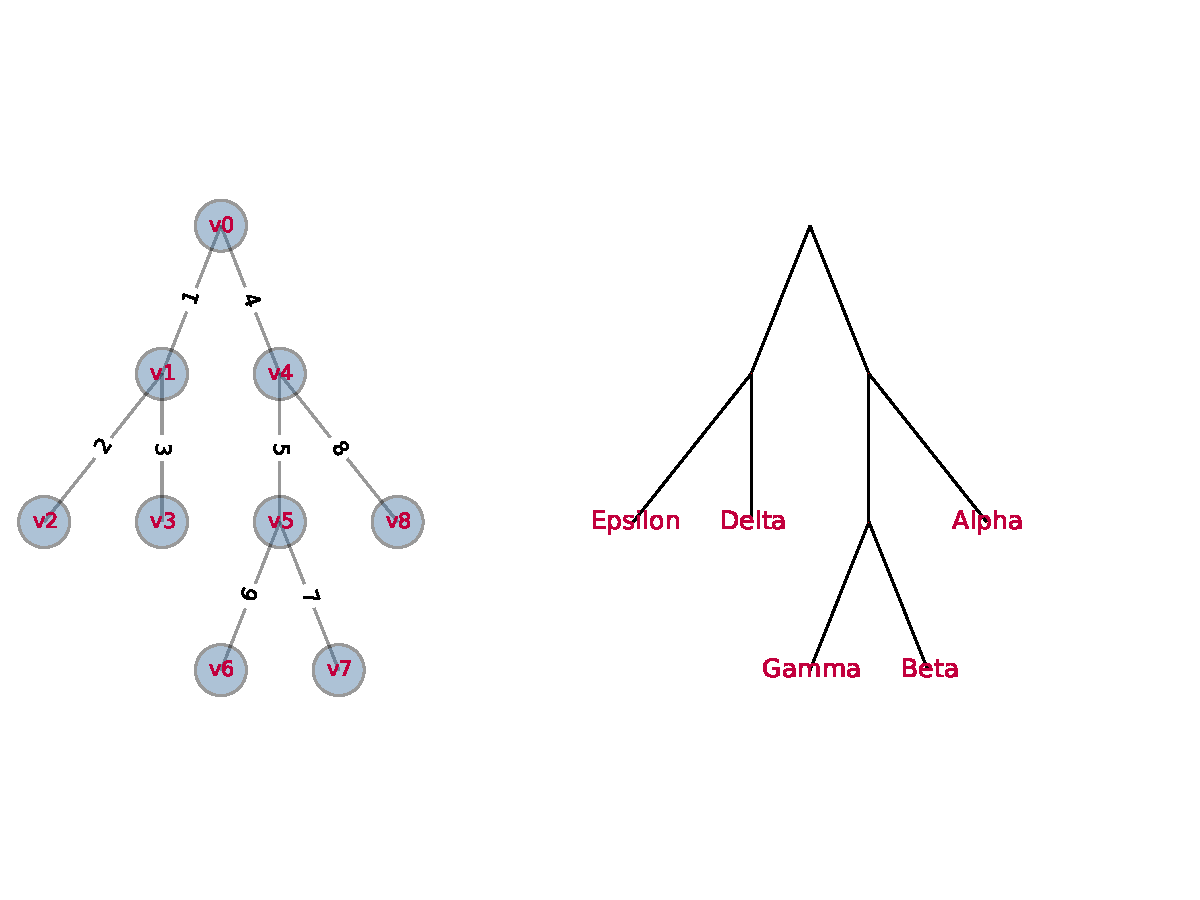
\includegraphics[scale=0.74, clip=true, trim=0 3cm 3cm 3cm]{gfx/tree_reconstruct_1.pdf}
	\end{center}
	\caption{Na levi strani je prikazan graf, ki je rekonstruiran iz vrednosti $P[j]$ iz slike \ref{img-reconstruct-m}. Da iz grafa pridobimo končno drevo, prikazano na desni strani, za označevanje listov uporabimo matriko $M'$ iz slike \ref{img-reconstruct-m}.}
	\label{img-reconstruct-1}
\end{figure}

\section{Vrednost asimetričnega srednjega drevesa}
Omenili smo že, da za en graf nekompatibilnosti lahko obstaja več največjih neodvisnih mnnožic in da to pomeni, da lahko sestavimo več različnih asimetričnih srednjih dreves. Prvotni razlog za uporabo konsenznih metod je iz večih dreves pridobiti eno drevo, zato potrebujemo metriko, s pomočjo katere se bomo lahko odločili za eno, najbolj podprto drevo.  

Najprej uvedemo utež binarnega niza $w(c_e)$ (\ref{eq:10}), ki je preprosto število dreves v vhodni množici $T$, ki vsebujejo binarni niz $c_e$. Vrednost asmetričnega srednjega drevesa $\tau$ glede na vhodno množico $T$ je določena (\ref{eq:11}) kot vsota uteži binarnih nizov, ki so prisotni v asimetričnem srednjem drevesu, vendar niso prisotni v vseh vhodnih drevesih (oz. striktnem konsenznem drevesu)\cite{pw}.

\begin{align}
	w(c_e) = \left| \left\{ i: c_e \in C(T_i) \right\} \right| \label{eq:10} \\
	value(T, \tau) = \sum_{c \in C(\tau) - \cap C(T_i)} w(c) \label{eq:11}
\end{align}

Najboljše najdeno asimetrično srednje drevo je tisto, ki maksimizira dano vsoto uteži \ref{eq:11}.

\section{Aproksimacijski algoritmi}
Ker je problem konstrukcije asimetričnega srednjega drevesa polinomsko prevedljiv na problem največje neodvisne množice\cite{pw} in zato za več kot dve drevesi sodi v razred NP-težkih problemov, je lahko izvajanje algoritma prepočasno, če imamo v vhodni množici $T$ veliko dreves. Zato si bomo ogledali dva aproksimacijska algoritma, ki imata polinomsko časovno zahtevnost.

Prvi, $\frac{2}{k}$-aproksimacijski algoritem, je enostaven. Za vsak par dreves $T_i, T_j \in T$ izračunamo asimetrično srednje drevo $\tau_{ij}$ in izberemo tistega, ki maksimizira vrednostno funkcijo $value(T, \tau_{ij})$. Ker je tako asimetrično srednje drevo sestavljeno iz dveh dreves, posledično lahko vsebuje le klade, ki so prisotne v teh dveh drevesih.

V kolikor imajo drevesa vhodne množice $T$ veliko skupnih klad, je primernejši drugi algoritem. Naj bo $V^* \subseteq V$ podmnožica vozlišč grafa nekompatibilnosti $I(V, E)$, in sicer tistih, ki so skupna vsem drevesom. Takih vozlišč v naslednjem koraku ne potrebujemo, saj niso povezana z nobenim drugim vozliščem. Nato izračunamo največje ujemanje (angl. maximum matching) v grafu $I(V - V^*, E)$, s čimer pridobimo množico robov $E_{M} \subseteq E$, ki nimajo skupnih vozlišč\cite{mgt}. Vozlišča $V_{M}$, ki so krajišča robov iz množice $E_{M}$, odstranimo iz množice $V$ in ostanejo nam le neujemajoča vozlišča $V_{N} = V - V_{M}$. Primer iskanja množice $V_N$ je prikazan na sliki \ref{img-maxmatch}. Iz binarnih nizov, pripadajočih vozliščem množice $V_{N}$, rekonstruiramo asimetrično srednje drevo po običanjem postopku. Tako drevo, za razliko od drevesa izračunanega s pomočjo prvega aproksimacijskega algoritma, lahko vsebuje klade iz večih dreves vhodne množice hkrati\cite{pw}. 

\begin{figure}
	\begin{center}
		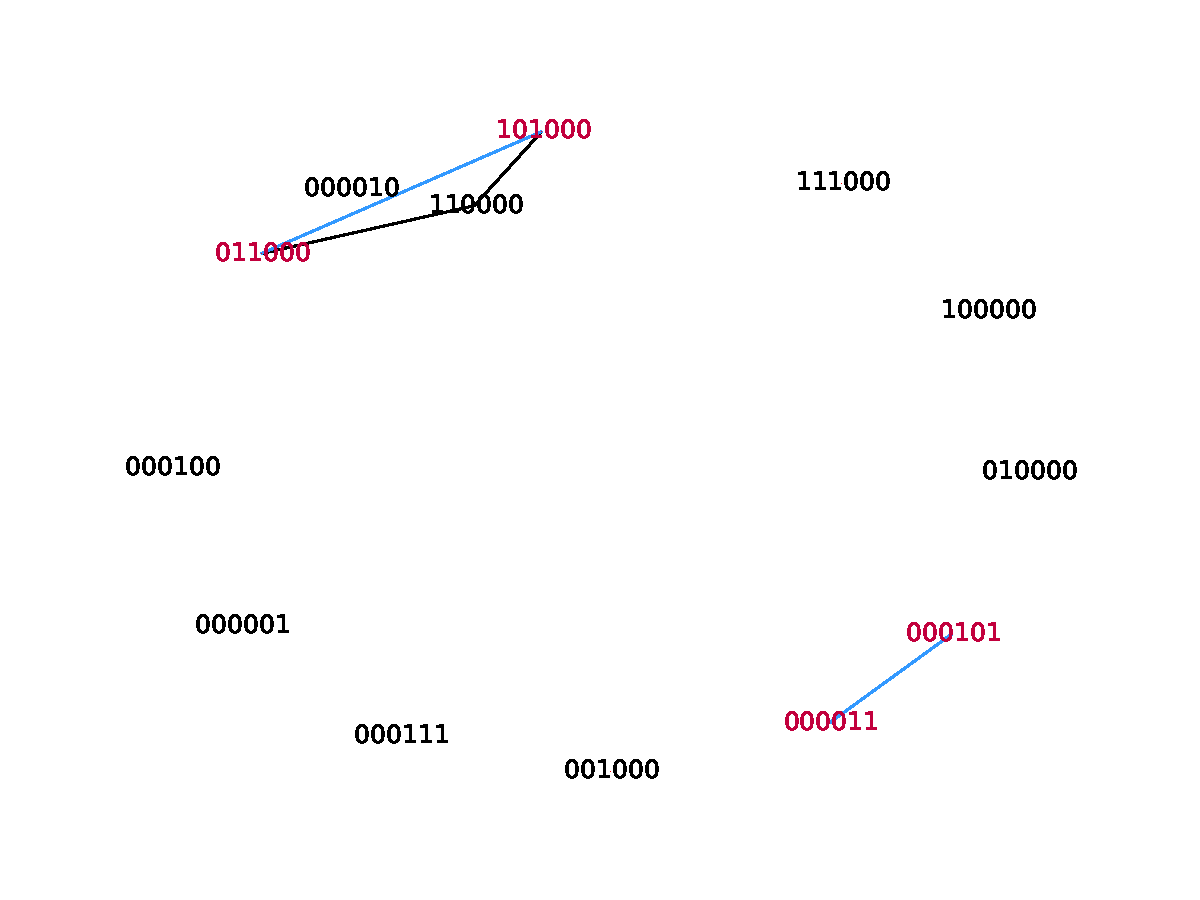
\includegraphics[scale=0.65, clip=true, trim=2cm 1cm 1cm 2cm]{gfx/maxmatch_graph.pdf}
	\end{center}
	\caption{Primer računanja bitnih nizov asimetričnega srednjega drevesa s pomočjo največjega ujemanja. Robovi, ki spadajo v množico največjega ujemanja $E_{M}$ so obarvani modro, njihova krajišča pa rdeče. Vsi bitni nizi, ki so obarvani črno, sestavljajo končno drevo.}
	\label{img-maxmatch}
\end{figure}

\chapter{Implementacija algoritma}

\section{Biopython}
Biopython\footnote{\url{http://biopython.org/}} je odprtokodni paket modulov, napisan v programskem jeziku Python, ki ponuja mnoge funkcionalnosti s področja bioinformatike. Olajša nam delo s formati datotek, kot so BLAST, ClustralW, FASTA ter GenBank in ponuja enostaven dostop do spletnih storitev, npr. NCBI\cite{biopy}. Poleg funkcionalnosti, implementiranih v programskem jeziku Python ponuja tudi enostaven dostop do zunanjih programov. Nekateri glavni moduli paketa Biopython, ki so relavantni tudi za računanje filogenetskih dreves, so: 

\begin{itemize}
	\item $Bio.SeqIO$: razredi, ki nam omogočajo branje, pisanje in manipuliranje sekvenc v različnih formatih ($FASTA$, $Nexus$, ...),
	\item $Bio.AlignIO$: razredi, ki nam omogočajo branje, pisanje in manipuliranje poravnanih sekvenc,
	\item $Bio.Application$: razredi, s pomočjo katerih enostavno dostopamo do zunanje namenske programske opreme, kot npr. PhyML in RAxML
	\item $Bio.Phylo$: razredi in funkcije za izračun filogenetskih dreves
\end{itemize} 

Modul $Bio.Phylo$ že omogoča izračun filogenetskih dreves s pomočjo metod UPGMA, Neighbor Joining in Maximum Parsimony. Poleg tega ponuja tudi metode ponovnega vzorčenja bootstrap in jackknife.  

Izračun konsenznih filogenetskih dreves je mogoč s pomočjo podmodula $Bio.Phylo.Consensus$ v katerem so bile najprej implementirane metode striktnega, večinskega in adamovega konsenza, sedaj pa izračun lahko opravimo tudi s pomočjo metode asimetričnega srednjega drevesa. Branje in pisanje dreves je že omogočeno za formate Newick, CDAO in PhyloXML. Modul ponuja tudi vmesno reprezentacijo drevesa, ki ga uporabljamo med izračunom in ni vezan na končni format.

\section{Podrobnosti implementacije}
Glavna entiteta, ki je nastopala v obravnavi metode asimetričnega srednjega drevesa je bil bitni niz. Zato je pomembno, da zanj uporabimo primerno hitro podatkovno strukturo. Razred, ki podatkovno strukturo že implementira se imenuje $\_BitString$, prebiva pa v podmodulu $Bio.Phylo.Consensus$. $\_BitString$ razširja Pythonovo vgrajeno podatkovno strukturo $String$, zato ga lahko uporabljamo na enak način. Med operatorji, ki jih lahko izvajamo nad podatkovno strukturo, so konjunkcija, disjunkcija in ekskluzivna disjunkcija nad posameznimi mesti, vsebuje pa tudi metodi za preverjanje vsebovanosti enega bitnega niza v drugem in preverjanje kompatibilnosti dveh binarnih nizov. 

Modul $Bio.Phylo$ za izrisovanje filogenetskih dreves uporablja paket networkx\footnote{\url{https://networkx.github.io/}}. Ta poleg samega izrisovanja ponuja tudi konstrukcijo grafov in njihovo nadaljno manipulacijo. Na grafu zmore izračunati aproksimacijo največje neodvisne množice, a se s tem nismo mogli zadovoljiti, saj je bila aproksimacija že za majhna vhodna drevesa preveč nenatančna, da bi dobili uporaben rezultat. Zato smo za konstrukcijo grafa in iskanje največje neodvisne množice vozlišč izbrali paket igraph\footnote{\url{http://igraph.org/python/}}, ki zmore najti vse največje neodvisne množice v danem grafu nekompatibilnosti. Čeprav smo s tem vnesli dodatno odvisnost od zunanjih paketov, lahko odločitev utemeljimo s precej večjo hitrostjo implementacije algoritmov paketa igraph v primerjavi z lastno implementacijo v programskem jeziku Python. Pri uporabi druge aproksimacijske metode za izračun asimetričnega srednjega drevesa pa ne računamo največje neodvisne množice, temveč največje ujemanje, za kar smo uporabili paket networkx, saj paket igraph zmore najti največje ujemanje le na bipartitnih grafih, naš graf inkompatibilnosti pa ima v splošnem lahko poljubno število particij.

Za rekonstrukcijo drevesa smo potrebovali orodje, ki je zmožno dela z matrikami. Ker je paket Biopython že odvisen od paketa numpy\footnote{\url{http://www.numpy.org/}}, je ta bil logična izbira. Med kreiranjem matrike je bilo potrebno binarne nize pretvoriti v stolpce matrike. Za to potrebo smo razredu \_BitString dodali metodo $to\_numpy()$, katera niz ničel in enic pretvori v binarni vektor tipa $numpy.ndarray$ z eno dimenzijo. Za potrebe sortiranja smo razredu $\_BitString$ dodali še metodo $\_\_int\_\_()$, ki izračuna desetiško vrednost binarnega niza.

Figura \ref{code-amt-func} prikazje glavo implementirane funkcije, ki se nahaja v modulu {\it Bio.Phylo.Consensus}. Opis parametrov funkcije se nahaja v tabeli \ref{table-amt-head}. Privzeto metoda izračuna točno asimetrično srednje drevo, vendar je računska kompleksnost za več kot dve drevesi eksponentna, zato lahko uporabnik, v kolikor to želi, z drugim parametrom izbere eno izmed aproksimacijskih metod. 

\begin{python}[label={code-amt-func}, caption={Glava funkcije za izračun asimetričnega srednjega drevesa iz modula {\it Bio.Phylo.Consensus}.}]
def amt_consensus(trees, method='no_approx')
\end{python}

\begin{table}
	\begin{center}
	{\footnotesize
    \begin{tabular}{ >{\centering}m{1.7cm} | >{\centering}m{2.9cm} | >{\centering}m{2.6cm} | >{\centering}m{4cm} } 
    Parameter & Tip                             & Vrednost parametra                        & Opis   \tabularnewline
    \hline
    trees     & seznam objektov tipa {\it BaseTree.Tree}           & /                            & Seznam vhodnih dreves v kateremkoli formatu, ki ga podpira Biopython.  \tabularnewline
    \hline
    \hline
    method    & niz                             &  ~                                         & Parameter za izbiro metode izračuna.  \tabularnewline
    ~         & ~                               & {\it no\_approx}                            & Izračun točnega drevesa.  \tabularnewline
    ~         & ~                               & {\it bi\_approx}                            & Izračun iz največ dveh dreves.  \tabularnewline
    ~         & ~                               & {\it maxmatch\_approx}                      & Izračun s pomočjo največjega ujemanja.  \tabularnewline
    \hline
    \end{tabular}
    }
    \caption{Opis parametrov in njihovih vrednosti metode {\it Bio.Phylo.Consensus.amt\_consensus.}}
    \label{table-amt-head}
	\end{center}    
\end{table}

\section{Primer uporabe}
Primer uporabe programske kode je najbolj enostavno prikazati na primeru. Recimo, da imamo pripravljeno datoteko (\ref{trees-input}) z imenom $primer\_a.tre$, ki vsebuje pet dreves v formatu Newick. Iz teh dreves želimo izračunati asimetrično srednje drevo in ga izrisati.

\begin{lstlisting}[label={trees-input}, caption={Primer petih polno razrešenih filogenetskih dreves s šestimi taksonomskimi enotami.}]
             ((A, (B, C)), (D, (E, F)));
             ((B, (A, C)), (D, (E, F)));
             ((A, (B, C)), (E, (D, F)));
             ((B, (A, C)), (E, (D, F)));
             ((C, (B, A)), (E, (D, F)));
\end{lstlisting}

Uporaba konsenzne metode asimetričnega srednjega drevesa v paketu Biopython je enostavna. Figura \ref{amt-example} predstavlja osnoven primer uporabe. V prvi vrstici uvozimo modul $Bio.Phylo$, v drugi iz podmodula $Bio.Phylo.Consensus$ uvozimo funkcijo $amt\_consensus$,  v tretji pa uvozimo paket za risanje $pyplot$.


V peti vrstici uvozimo filogenetska drevesa iz datoteke $primer\_a.tre$ in jih razčlenimo, s čimer dobimo seznam objektov tipa $Bio.Phylo.BaseTree.Tree$. V šesti vrstici s preprostim klicem funkcije iz obstoječega seznama dreves izračunamo asimetrično srednje drevo. V sedmi vrstici drevo preoblikujemo tako, da bodo globlja poddrevesa prikazana na vrhu, in v zadnjih dveh vrsticah drevo izrišemo na ekran. 

Rezultat je programa iz figure \ref{amt-example} je prikazan na sliki \ref{img-example-output}. Poleg drevesa so prikazane še osi, ki v našem primeru sicer niso pomembne, v splošnem pa iz osi x lahko razberemo divergentne čase taksonomskih enot. \\\\

\begin{python}[label={amt-example}, caption=Primer programske kode za branje dreves iz datotek in izračun asimetričnega srednjega drevesa.]
	from Bio import Phylo
	from Bio.Phylo.Consensus import amt_consensus
	from matplotlib import pyplot
	
	trees = list(Phylo.parse('primer_a.tre', 'newick'))
	amt = amt_consensus(trees)
	amt.ladderize()
	Phylo.draw(amt)
	pyplot.show()
\end{python}

\begin{figure}[h!]
	\begin{center}
		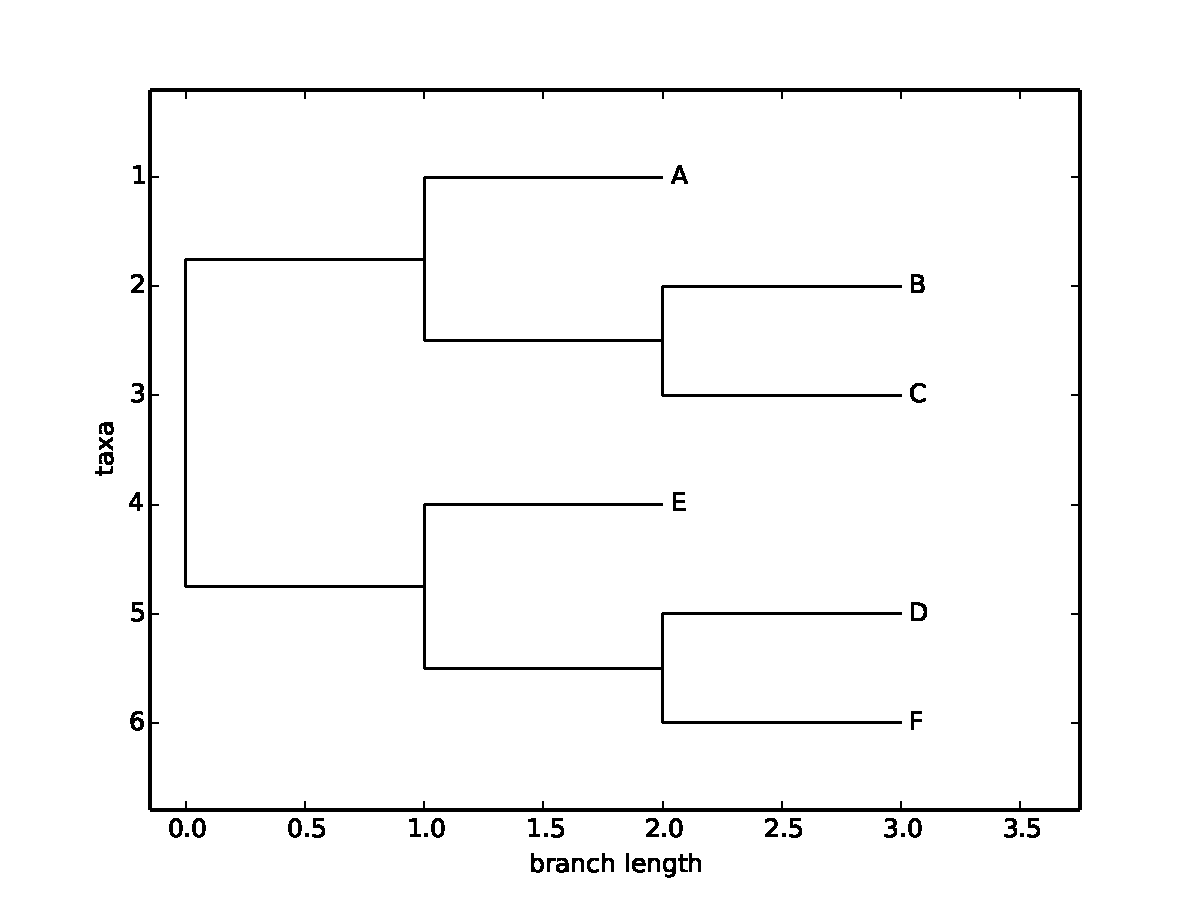
\includegraphics[scale=0.65, clip=true, trim=1cm 0 1cm 1cm]{gfx/ex_b.pdf}
	\end{center}
	\caption{Rezultat programa iz figure \ref{amt-example}.}
	\label{img-example-output}
\end{figure}

\chapter{Eksperimentalna primerjava}

Vse tri implementirane metode računanja asimetričnega srednjega drevesa želimo primerjati med sabo in glede na metode striktnega, večinskega in adamovega konsenza. Za ta namen smo pripravili nekaj vhodnih množic in jih preizkusili glede na razrešenost končnega drevesa ter glede na Robinson-Fouldsovo metriko. Poleg lastnosti izhodnih dreves nas je zanimal tudi čas izvajanja vseh treh implementiranih metod, s čimer smo ocenili velikost vhodne množice in število taksonomskih enot v drevesih, za katere zaradi predolgega časa izvajanja ni več smiselno uporabiti  natančne metode. 

\section{Razrešenost drevesa in Robinson-Fouldsova metrika}
Razrešenost drevesa (\ref{eq:res}) je definirana kot število povezav, ki nastopajo v drevesu. Ker imajo vsa drevesa enako število listov, se je drevo z največjim številom povezav največkrat razvejalo. Najbolj razrešeno drevo je binarno drevo (takrat rečemo, da je {\it polno razrešeno}). To ponuja največ informacije o evolucijski zgodovini, saj za vsak par taksonomskih enot vemo, iz katerega skupnega prednika sta se enoti razvili. Zaželjeno je torej, da je število povezav v drevesu čim večje.

\begin{align}
	Res(T) = \left|E(T)\right| \label{eq:res} ~~~~~~~~~~~~~~~~~~~~~ \\
	RF(T_1, T_2) = \left|C(T_1) - C(T_2)\right| + \left|C(T_2) - C(T_1)\right|  \label{eq:rf}
\end{align}

Robinson-Fouldsova (RF) metrika je najbolj razširjena metrika za primerjanje filogenetskih dreves. Šteje število klad (\ref{eq:rf}), ki si jih drevesi ne delita\cite{rf}. Za izračun vrednosti RF smo uporabili funkcijo {\it symmetric\_difference()} iz paketa DendroPy\footnote{\url{https://pythonhosted.org/DendroPy/}}, saj v paketu Biopython RF metrika še ni implementirana. Vrednost RF smo izračunali za vsak par konsenznega in vhodnega drevesa, ter za vsako konsenzno drevo vrednosti RF sešteli.

\section{Vhodna množica 1}
\begin{figure}[h!]
	\begin{center}
		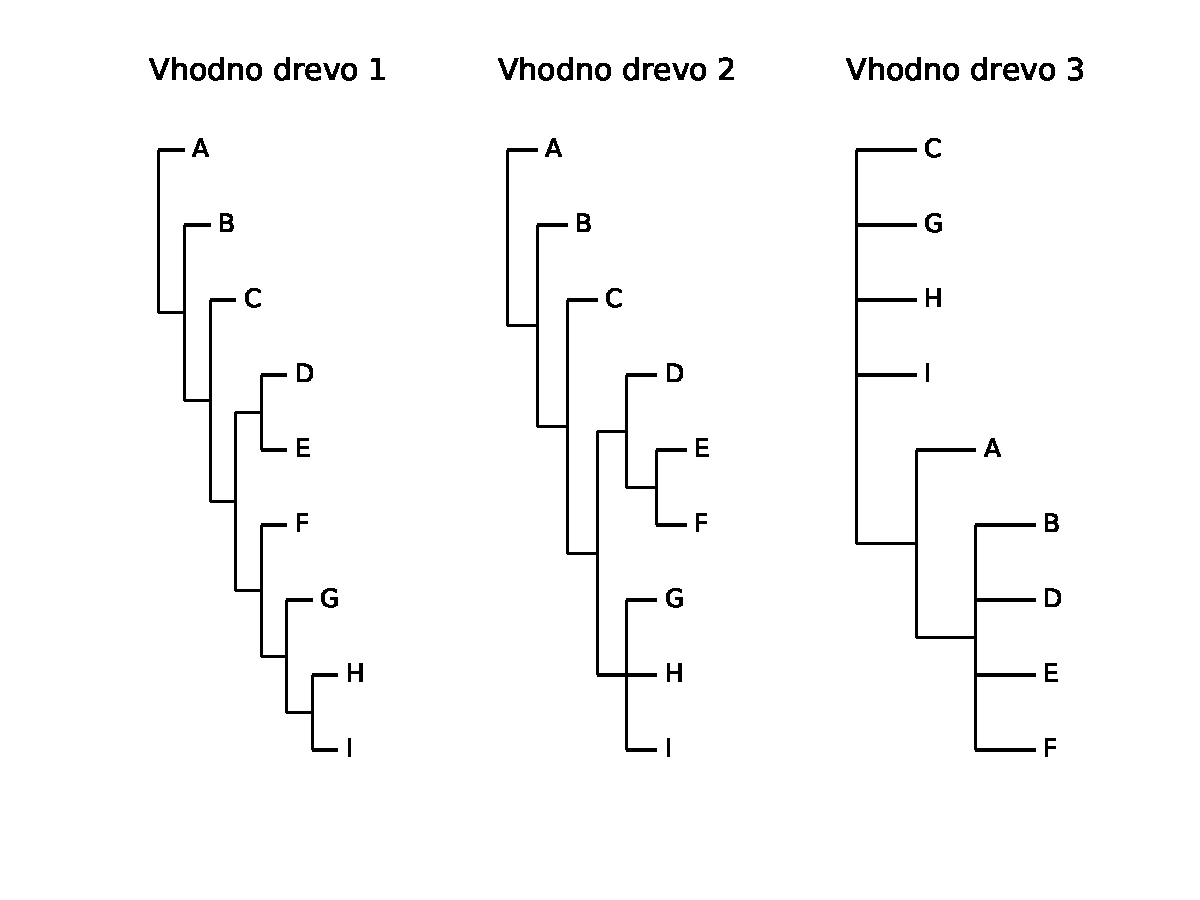
\includegraphics[scale=0.45, clip=true, trim=1cm 2cm 1cm 0]{gfx/eval_input.pdf}
	\end{center}
	\caption{Prva vhodna množica dreves.}
	\label{img-eval-input}
\end{figure}

\begin{table}
	\begin{center}
	{\footnotesize
	\begin{tabular}{ l| l | l | l | l | l }
	~                & Res ($T$) & RF ($T_1$) & RF ($T_2$) & RF ($T_3$) & RF (vsota) \\ \hline
	AMT              & 17          & 4             & 1             & 8             & 13         \\ \hline
	Bi-AMT           & 16          & 5             & 0             & 7             & 12         \\ \hline
	MM-AMT           & 13          & 3             & 4             & 5             & 12         \\ \hline
	Striktni konsenz & 10          & 6             & 5             & 2             & 13         \\ \hline
	Večinski konsenz & 17          & 2             & 5             & 4             & 11         \\ \hline
	Adamov konsenz   & 17          & 2             & 5             & 4             & 11         \\ \hline
	\end{tabular}
	\caption{Razrešenost konsenznih dreves in njihove RF vrednosti za vhodna drevesa na sliki (\ref{img-eval-input}).}
	}
	\label{table-eval-1}
	\end{center}		
\end{table}

Tabela (\ref{table-eval-1}) prikazuje razrešenost in RF vrednosti asimetričnega srednjega drevesa, dveh aproksimiranih asimetričnih srednjih dreves (Bi-AMT in MM-AMT), striktnega, večinskega in adamovega konsenznega drevesa iz slike (\ref{img-eval-result}) glede na vhodna drevesa iz slike (\ref{img-eval-input}). Opazimo, da je asimetrično srednje drevo glede na razrešenost prav tako dobro kot drevesi večinskega in adamovega konsenza. Vsa ta drevesa so polno razrešena. Glede na vrednosti RF sta vhodnim drevesom najbolj podobni večinsko in adamovo konsenzno drevo. Ti dve drevesi lahko razglasimo za najboljši drevesi za prvo vhodno množico.

\begin{figure}[h!]
	\begin{center}
		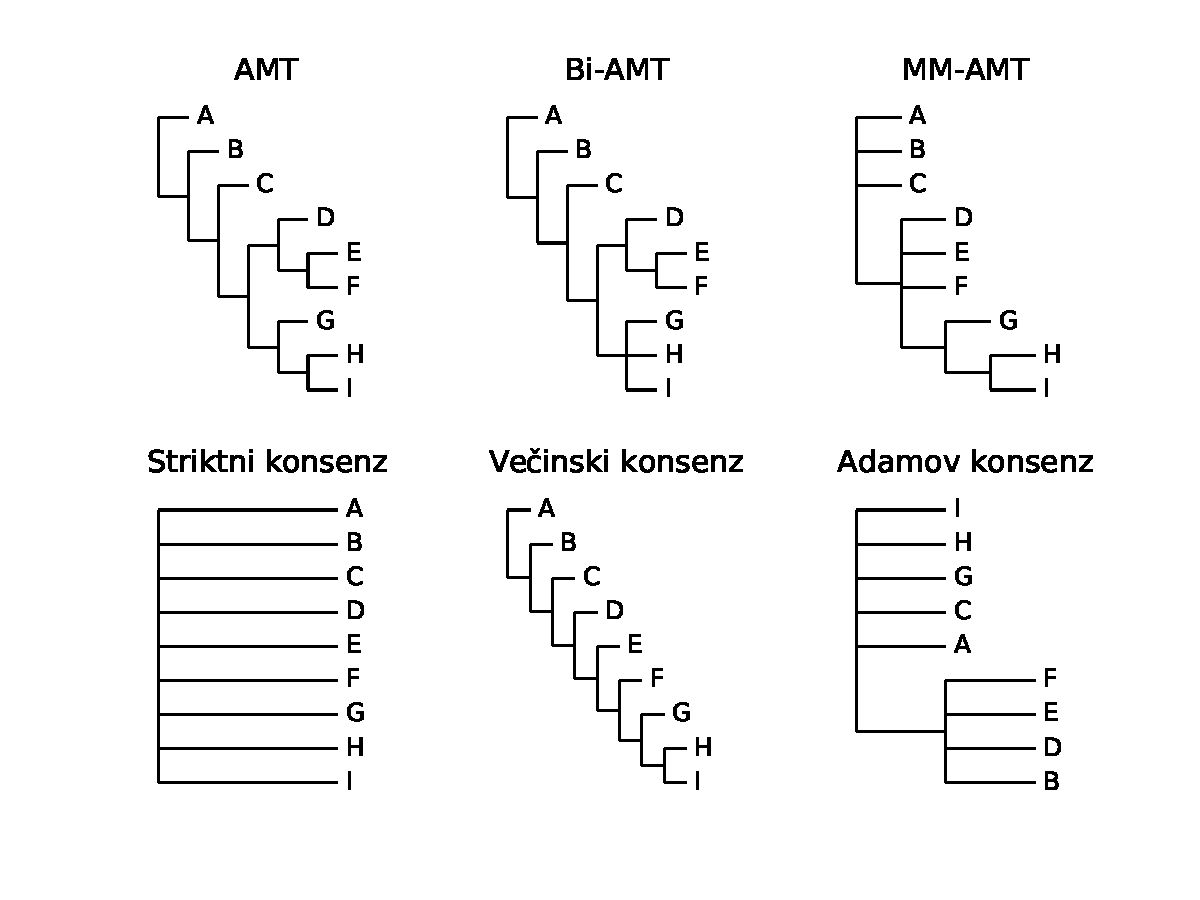
\includegraphics[scale=0.55, clip=true, trim=1.5cm 1.5cm 1cm 0.8cm]{gfx/eval_gfx.pdf}
	\end{center}
	\caption{Konsenzna drevesa, zgrajena iz množice dreves na sliki (\ref{img-eval-input}). Oznaka Bi-AMT označuje približek asimetričnega srednjega drevesa zgrajenega iz dveh vhodnih dreves, MM-AMT pa aproksimirano drevo zgrajeno s pomočjo največjega ujemanja.}
	\label{img-eval-result}
\end{figure}

Rezultat je pričakovan, saj je večina klad prisotna v več kot polovici vhodnih dreves, preostale pa so povečini medsebojno kompatibilne, kar je za večinsko in adamovo drevo ugodno. Najbolj podobno asimetrično srednje drevo je MM-AMT, vendar je njegova razrešenost med najslabšimi. Drevo Bi-AMT ne podaja informacije o skupnem predniku taksonomskih enot $H$ in $I$, zaradi česar je bolj podobno drugemu in tretjemu vhodnemu drevesu kot drevo AMT, posledično pa je njegova razrešenost zaradi tega slabša. 

\section{Vhodna množica 2}
\begin{figure}[h!]
	\begin{center}
		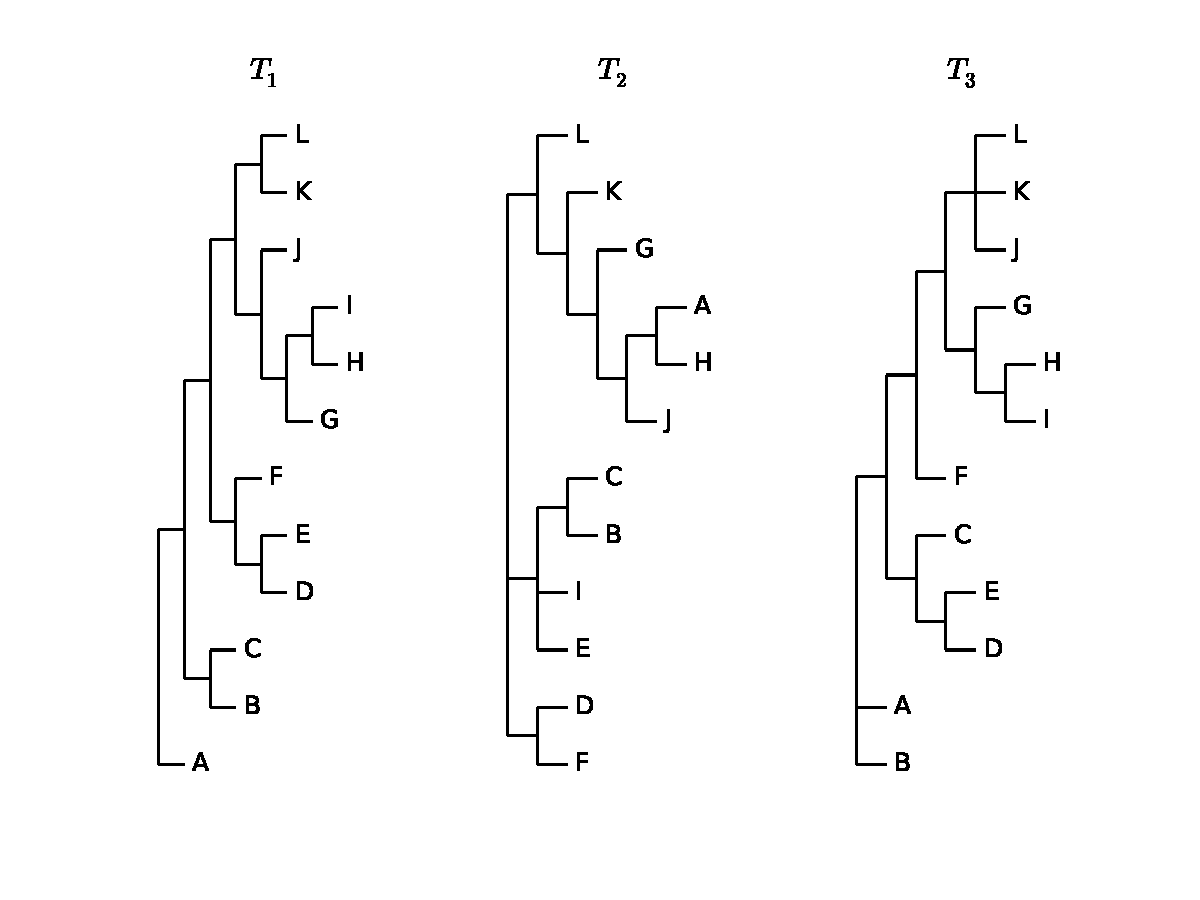
\includegraphics[scale=0.50, clip=true, trim=1cm 2cm 1cm 0]{gfx/eval_input_2.pdf}
	\end{center}
	\caption{Druga vhodna množica dreves.}
	\label{img-eval-input-2}
\end{figure}

\begin{table}[h!]
	\begin{center}
	{\footnotesize
	\begin{tabular}{ l| l | l | l | l | l }
	~                & Res ($T$) & RF ($T_1$) & RF ($T_2$) & RF ($T_3$) & RF (vsota) \\ \hline
	AMT              & 23          & 12            & 9             & 7             & 28         \\ \hline
	Bi-AMT           & 22          & 10            & 11            & 11            & 32         \\ \hline
	MM-AMT           & 15          & 9             & 6             & 6             & 21         \\ \hline
	Striktni konsenz & 15          & 7             & 8             & 8             & 23         \\ \hline
	Večinski konsenz & 23          & 10            & 11            & 9             & 30         \\ \hline
	Adamov konsenz   & 23          & 10            & 11            & 9             & 30         \\ \hline
	\end{tabular}
	\caption{Razrešenost konsenznih dreves in njihove RF vrednosti za vhodna drevesa na sliki (\ref{img-eval-input-2}).}
	}
	\label{table-eval-2}
	\end{center}		
\end{table}



Rezultati konsenznih dreves iz slike (\ref{img-eval-result-2}) glede na vhodna drevesa iz slike (\ref{img-eval-input-2}) so prikazani v tabeli (\ref{table-eval-2}). Ponovno so asimetrično srednje drevo ter drevesi večinskega in adamovega konsenza polno razrešena. Če ta drevesa medsebojno primerjamo še po podobnosti vhodnim drevesom, se je najbolje odrezalo asimetrično srednje drevo. Čeprav sta striktno konsenzno drevo in drevo MM-AMT enako slabo razrešeni, je drevo MM-AMT bolj podobno vhodnim drevesom. Drevo Bi-AMT je sicer dobro razrešeno, vendar 
najmanj podobno vhodnim drevesom. 

\begin{figure}[h!]
	\begin{center}
		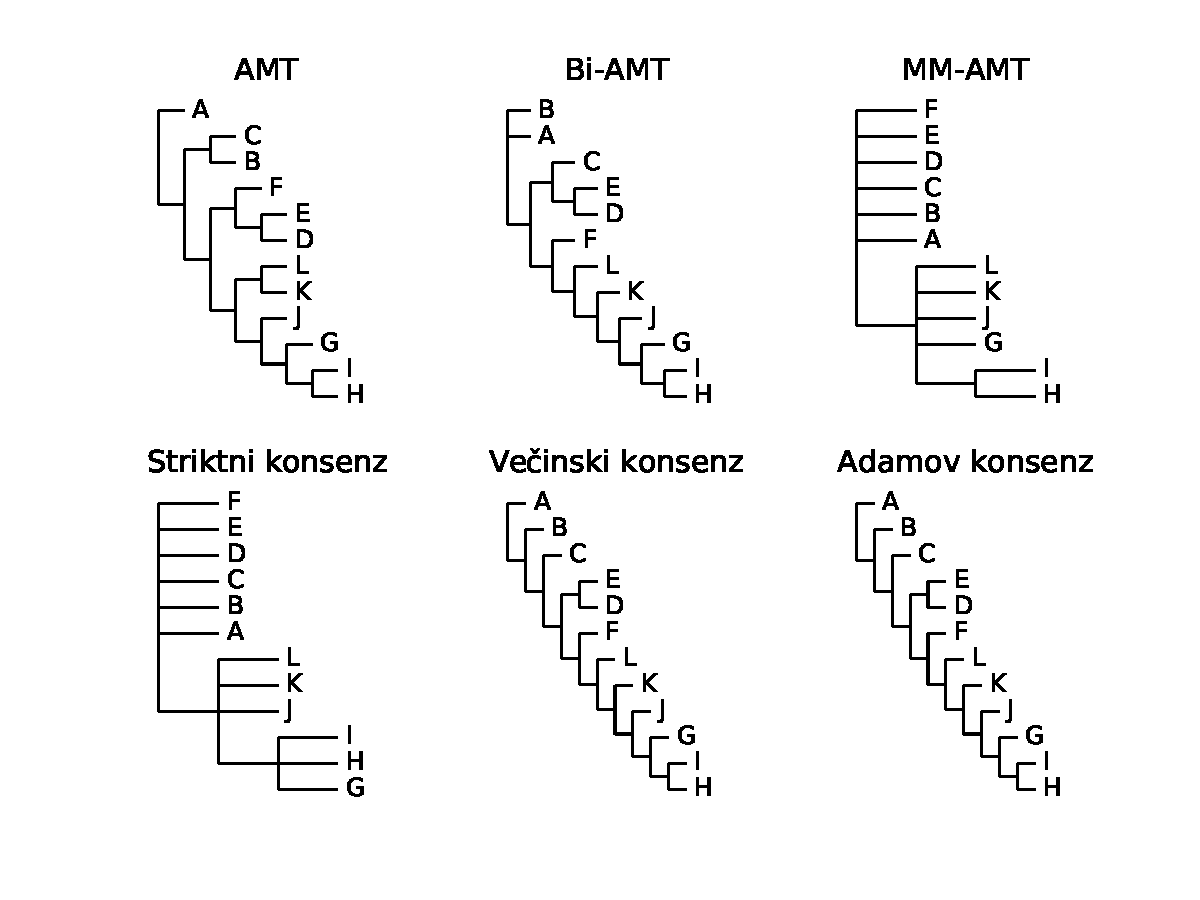
\includegraphics[scale=0.65, clip=true, trim=1.5cm 1.5cm 1cm 0.8cm]{gfx/eval_gfx_2.pdf}
	\end{center}
	\caption{Konsenzna drevesa, zgrajena iz množice dreves na sliki (\ref{img-eval-input-2}).}
	\label{img-eval-result-2}
\end{figure}

Ker večina klad ni prisotna v več kot polovici vhodnih dreves, večinoma pa so medsebojno kompatibilne, je rezultat pričakovan. Slaba razrešenost drevesa MM-AMT je najverjetneje posledica majhnega števila skupnih klad in majhnega števila vhodnih dreves.   

\section{Vhodna množica 3}
\begin{figure}[h!]
	\begin{center}
		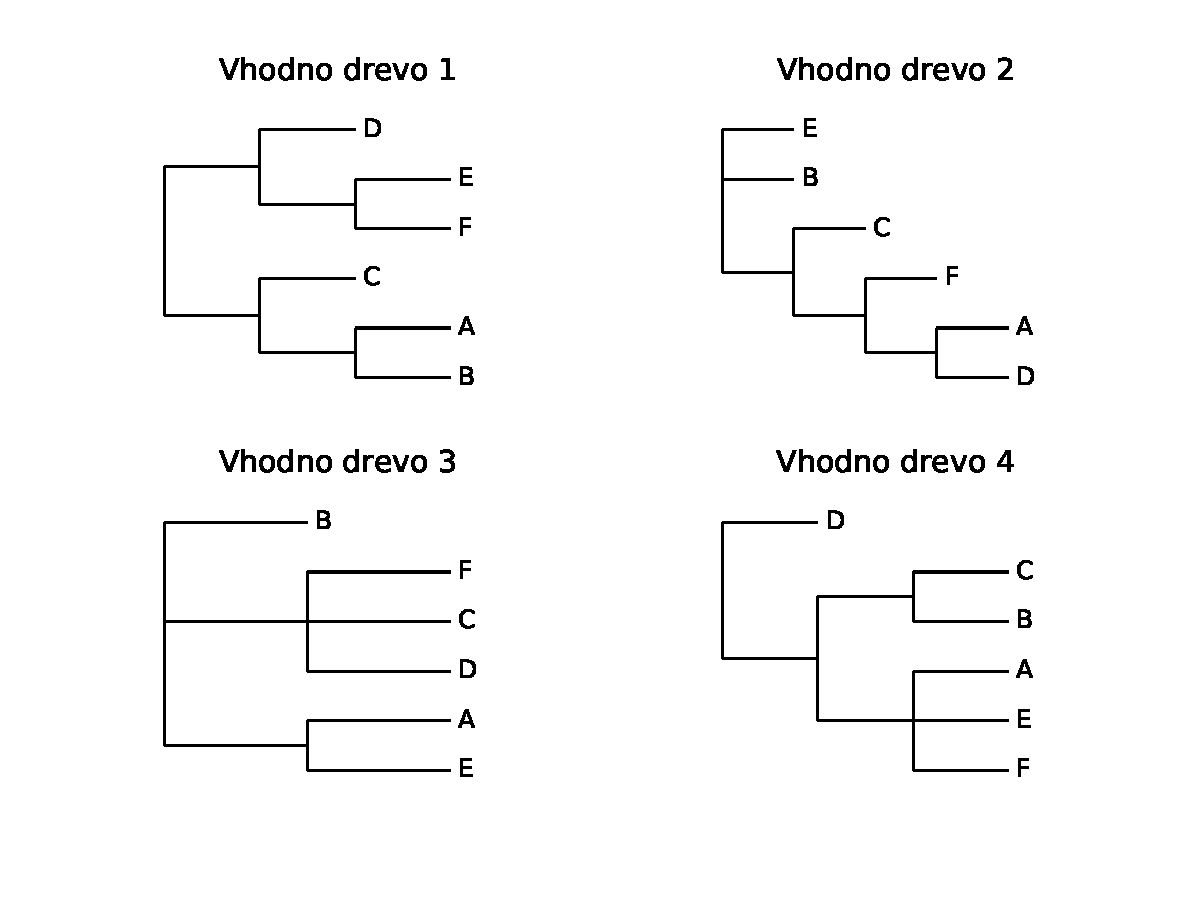
\includegraphics[scale=0.63, clip=true, trim=0 2cm 0 0.5cm]{gfx/eval_input_3.pdf}
	\end{center}
	\caption{Tretja vhodna množica dreves.}
	\label{img-eval-input-3}
\end{figure}

Zadnja, tretja vhodna množica dreves iz slike \ref{table-eval-3}, je sestavljena tako, da je število skupnih klad majhno, posamezne klade ne nastopajo v več kot polovici vhodnih dreves in so večinoma medsebojno nekompatibilne. Rezultate dobljenih konseznih dreves na sliki (\ref{img-eval-input-3}) prikazuje tabela (\ref{img-eval-result-3}).

\begin{table}[h!]
	\begin{center}
	{\footnotesize
	\begin{tabular}{ l| l | l | l | l | l | l }
	~                & Res (T)      & RF ($T_1$) & RF ($T_2$)       & RF ($T_3$) & RF($T_4$) & RF (vsota) \\ \hline
	AMT              & 11          & 0          & 2                & 3          & 1         & 6          \\ \hline
	Bi-AMT           & 11          & 0          & 2                & 3          & 1         & 6          \\ \hline
	MM-AMT           & 7           & 3          & 3                & 2          & 2         & 10         \\ \hline
	Striktni konsenz & 7           & 3          & 3                & 2          & 2         & 10         \\ \hline
	Večinski konsenz & 10          & 0          & 2                & 3          & 1         & 6          \\ \hline
	Adamov konsenz   & 10          & 0          & 2                & 3          & 1         & 6          \\ \hline
	\end{tabular}
	\caption{Razrešenost konsenznih dreves in njihove RF vrednosti za vhodna drevesa na sliki (\ref{img-eval-input-3}).}
	}
	\label{table-eval-3}
	\end{center}		
\end{table}

Opazimo, da sta polno razrešeni le asimetrično srednje drevo in aproksimirano drevo Bi-AMT. Vsa ostala drevesa vsebujejo vsaj eno nerazrešeno vozlišče. Drevo MM-AMT je v tem primeru enako striktnemu konsenznemu drevesu, tako po topologiji kot glede na razrešenost in RF metriko. Preostala drevesa so glede na RF metriko sicer enakovredna, vendar ker drevesi večinskega in adamovega konsenza nista polno razrešeni, lahko za najboljši drevesi razglasimo asimetrično srednje drevo in Bi-AMT drevo, ki sicer nimata popolnoma enakih topologij.

Slaba razrešenost drevesa MM-AMT je ponovno posledica majhnega števila skupnih klad in v takem primeru je aproksimacija Bi-AMT boljša. Ker posamezne klade ne nastopajo v več kot polovici vhodnih dreves, metodama striktnega in adamovega konsenza ni uspelo popolnoma razrešiti vseh vozlišč vhodnih dreves, saj so klade s premalo pojavitvami kaznovane. Asimetrično srednje drevo za razliko take klade vključi, če to doprinese k informiranosti drevesa.

\begin{figure}
	\begin{center}
		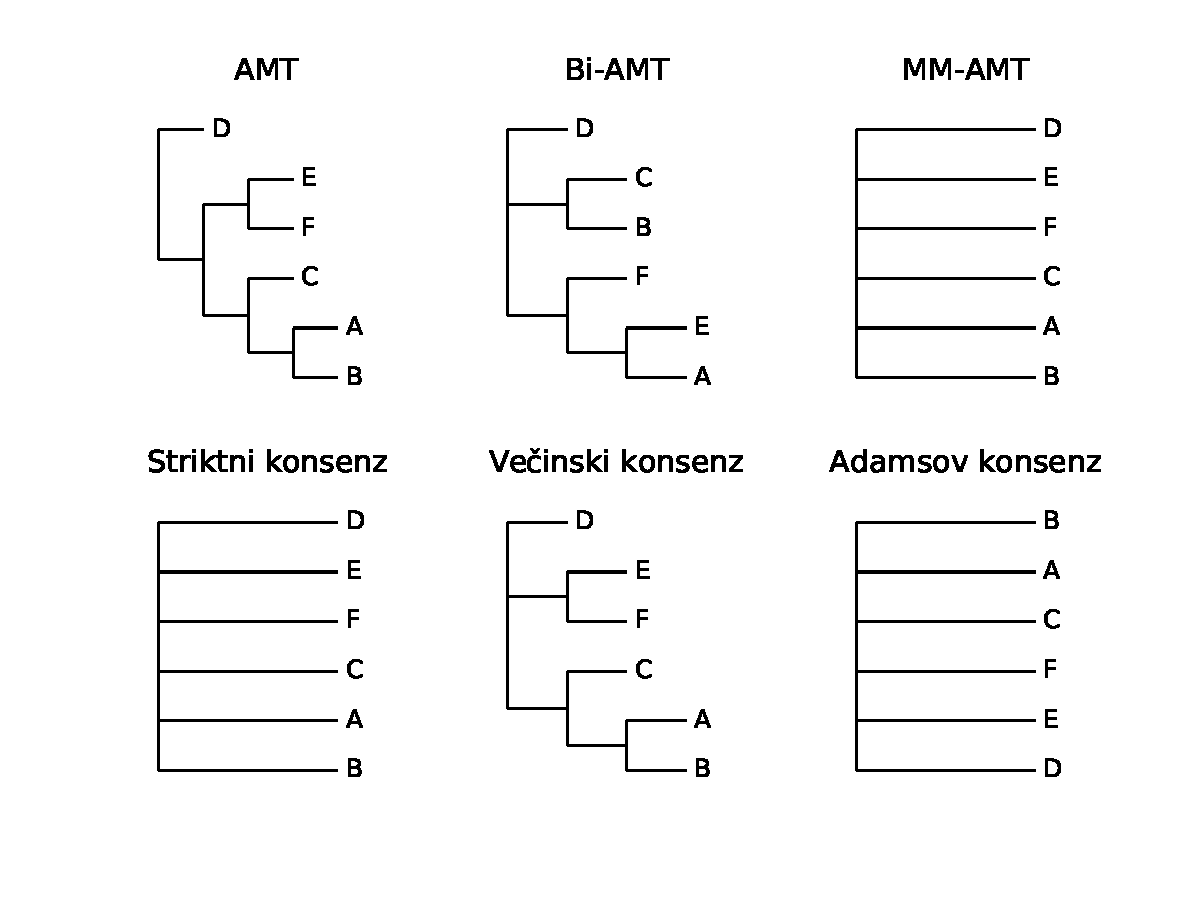
\includegraphics[scale=0.6, clip=true, trim=1.5cm 1.5cm 1cm 0.8cm]{gfx/eval_gfx_3.pdf}
	\end{center}
	\caption{Konsenzna drevesa, zgrajena iz množice dreves na sliki (\ref{img-eval-input-3}).}
	\label{img-eval-result-3}
\end{figure}

Razlika med asimetričnim srednjim drevesom in aproksimiranim drevesom Bi-AMT ni tako očitna, ker je vhodna množica majhna. Drevo Bi-AMT je namreč zgrajeno le iz dveh vhodnih dreves in v kolikor bi vhodno množico povečali, bi postale razlike bolj očitne, saj bi bilo asimetrično srednje drevo za razliko od približka sposobno vključiti informacije iz večih dreves hkrati.

\section{Primerjava izvajalnih časov}
Zaradi eksponentne časovne kompleksnosti metode asimetričnega srednjega drevesa nas zanima, kako velika drevesa lahko v doglednem času še izračunamo. Merjenje izvajalnega časa smo opravili na dvojedrnem procesorju i5-3200M, pri čemer smo izrabili le eno jedro, ki teče na frekvenci 1.7 GHz.

Hitrost računanja je odvisna od dveh parametrov, in sicer števila dreves v vhodni množici in števila taksonomskih enot, ki so v drevesih zastopane.

\begin{table}[h!]
	\begin{center}
	{\footnotesize
	\begin{tabular}{ l| l | l | l | l }
	Št. dreves       & Št. taksonomskih enot & AMT [$s$] & Bi-AMT [$s$] & MM-AMT [$s$] \\ \hline
	5                & 5                     & $0.017$   & $0.058$      & $0.020$      \\ \hline
	5                & 10                    & $0.119$   & $0.339$      & $0.146$      \\ \hline
	5                & 20                    & $1.252$   & $1.641$      & $0.904$      \\ \hline
	5                & 22                    & $6.321$   & $2.121$      & $1.255$      \\ \hline
	5                & 25                    & $26.448$  & $2.789$      & $1.085$      \\ \hline
	5                & 28                    & $163.676$ & $3.753$      & $1.509$      \\ \hline
	5                & 31                    & $527.254$ & $4.712$      & $1.760$      \\ \hline
	20               & 5                     & $0.043$   & $1.091$      & $0.045$      \\ \hline
	20               & 9                     & $2.340$   & $4.912$      & $0.740$      \\ \hline
	20               & 11                    & $18.915$  & $8.190$      & $3.334$      \\ \hline
	20               & 14                    & $421.215$ & $14.066$     & $7.456$      \\ \hline
	20               & 15                    & $3654.519$ & $17.084$    & $9.444$      \\ \hline
	\end{tabular}
	\caption{Časi izvajanja metode asimetričnega srednjega drevesa in obeh aproksimacijskih metod za različne velikosti vhodne množice in različnih števil taksonomskih enot.}
	}
	\label{table-timing-1}
	\end{center}		
\end{table}


\chapter{Zaključek}
Najpomembnejši rezultat dela je zagotovo prva znana implementacija konsenzne metode asimetričnega srednjega drevesa v programski paket Biopython. Čeprav je računska kompleksnost metode v splošnem eksponentna, kar je nezaželjeno, na probleme z izvajalnim časom nismo naleteli. V kolikor ta predstavlja oviro, ima uporabnik možnost izbire ene izmed aproksimacijskih metod. Pravilna izbira aproksimacijske metode je, kot smo pokazali tudi eksperimentalno, odvisna predvsem od lastnosti dreves v vhodni množici. 

Kot smo pokazali na treh vhodnih množicah, asimetrično srednje drevo ni nujno tisto, ki drevesa vhodne množice povzema najbolje. Prav tako kot z izbiro aproksimacijske metode tudi tukaj velja, da je izbira konsenzne metode odvisna predvsem od predhodnega poznavanja lastnosti dreves vhodne množice. V kolikor ta vsebujejo veliko število nekompatibilnih parov poddreves, potem je izbira metode asimetričnega srednjega drevesa smotrna, v nasprotnem primeru pa lahko že večinsko ali adamovo konsenzno drevo da primerljive, če ne celo boljše rezultate.

Kar se tiče razrešenosti dreves, je v naših testnih primerih asimetrično srednje drevo vedno bilo polno razrešeno in tako ponujalo največ informacije o evolucijski zgodovini, s čimer je prekašalo vse ostale metode. Tega sicer ne moremo trditi za obe aproksimacijski metodi. Metoda z izračunom največjega ujemanja je po razrešenosti v nekaterih primerih bila primerljiva zgolj s striktnim konsenznim drevesom, metoda z izračunom drevesa iz dveh vhodnih dreves pa je ob dobri razrešenosti običajno proizvedla drevo, ki se slabše ujema z vhodnimi drevesi.

Možnosti za izboljšave vidimo predvsem pri aproksimacijskih algoritmih. Nad drevesi, izračunanimi s pomočjo prvega aproksimacijskega algoritma, bi npr. lahko ponovno izračunali konsenzna drevesa in izbrali najboljšega. Prav tako so potrebne dodatne študije, s katerimi bi identificirali lastnosti dreves vhodne množice, za da metoda asimetričnega srednjega drevesa boljše rezultate.


\begin{thebibliography}{99}

\bibitem{cd}
C.\ Darwin. ``Notebook B: Transmutation of species'', str. 36, 1837-1838.

\bibitem{pw}
C.\ Phillips, T.\ J.\ Warnow. ``The asymmetric median tree - A new model for building consensus trees'', {\it Discrete Applied Mathematics}, št.\ 71, str.\ 311–335, 1996.

\bibitem{gd}
D. Gusfeld. ``Efficient algorithms for inferring evolutionary trees'', {\it Networks}, št. 21, str.\ 19-28, 1991.

\bibitem{fel}
J.\ Felsenstein. \textit{Inferring Phylogenies}. Sinauer Associates, 2004.

\bibitem{bw}
T.\ Y.\ Berger-Wolf. Properties of compatibility and consensus sets of phylogenetic trees. UNM Computer Science Technical Report, TR-CS-2004-24, 2004.

\bibitem{rf}
T.\ Asano, J.\ Jansson, K.\ Sadakane, R.\ Uehara, G.\ Valiente. ``Faster computation of the Robinson–Foulds distance between phylogenetic networks'', {\it Information Sciences}, št. 197, str.\ 77-90, 2012.

\bibitem{phy} 
Phylogenetics
dostopno na:\\ http://en.wikipedia.org/wiki/Phylogenetics

\bibitem{biopy}
Biopython tutorial and cookbook
dostopno na: \\ http://biopython.org/DIST/docs/tutorial/Tutorial.html

\bibitem{mgt}
Matching (Graph Theory)
dostopno na: \\ http://en.wikipedia.org/wiki/Matching\_(graph\_theory)


\end{thebibliography}

\end{document}

